\chapter{Base de données}


\boitemagique{Objectif}{Dans ce chapitre, nous appliquons MDFT sur une base de données de plus de 600 petites molécules plusieurs neutres afin d'en évaluer la pr\'ecision. Une étude détaillée de ces résultats ainsi obtenus nous permettrons d'orienter les futures développements de MDFT.}

Dans les chapitres précédents, nous avons testé et validé la théorie et son implémentation sur seulement quelques molécules modèles comme des sphères de Lennard-Jones. Dans ce chapitre, nous allons étudier un espace chimique plus large afin de mettre en évidence les points forts et faibles de MDFT et ainsi de pouvoir proposer des correctifs adaptés.



\section{La base de données FreeSolv}
Dans ce chapitre nous nous concentrerons sur la base de données mise à disposition par David Mobley et al. \cite{Mobley_small_2009} nommée FreeSolv. Elle est largement utilisée dans l'évaluation de méthodes de calcul d'énergie libres de solvatation. Elle est composée de 643 petites molécules neutres, accompagnées de nombreuses méta-données telles que leur énergie libre de solvatation expérimentale issue de la littérature, leur énergie libre de solvatation calculée par dynamique moléculaire et intégration thermodynamique ou encore les groupes chimiques qu'elles possèdent. Les paramètres quantitatifs sont accompagnés dès que possible de leur incertitude.

\subsection{Les molécules}
Lors de sa première publication, Freesolv, composée de 504 molécules, était le regroupement de la base de données de Rizzo et al\cite{Rizzo_estimation_2006} et de calculs précédemment effectués par David Mobley et ses collaborateurs. Depuis, David Mobley et al, ont concentré leurs efforts à la nettoyer\cite{Mobley_small_2009, Mobley_treating_2008, Mobley_comparison_2007, Mobley_predictions_2009, Beckstein_prediction_2011, Mobley_alchemical_2011, Mobley_blind_2014, Mobley_freesolv_2014, DuarteRamosMatos_approaches_2017} en supprimant les doublons, en vérifiant dans la littérature les valeurs des énergies libres de solvatation ou encore en essayant de peupler au mieux les zones sous représentées de l'espace chimique. Le nombre de composés est ainsi passé de 504 à 643 aujourd'hui. Ces molécules contiennent entre 3 et 44 atomes, pour des énergies libres de solvatation expérimentales allant de -25,47 à 3,43 $\mathrm{kcal}.\mathrm{mol}^{-1}$. 

\subsection{Les groupes chimiques}
Comme on le voit dans le tableau \ref{tab:freeSolvGroupNumbers}, un ensemble de 73 groupes chimiques sont plus ou moins représentés. Par exemple, nous comptons 267 composés aromatiques, 88 hétérocycles contre seulement 1 sulfoxyde ou 1 acide sulfurique diester. Parmi les 643 molécules qui composent FreeSolv, seules 38 n'appartiennent à aucun groupe. Cette catégorisation nous permet une analyse en profondeur des points forts et faibles de MDFT en fonction de chaque groupe chimique.



\csvautolongtable[separator=comma,
                    table head=\caption{Répartition des groupes chimiques présents dans FreeSolv}\label{tab:freeSolvGroupNumbers}\\\hline
                    \csvlinetotablerow\\\hline
                    \endfirsthead\hline
                    \csvlinetotablerow\\\hline
                    \endhead\hline
                    \endfoot,
                    respect all
                  ]{chapters/BDD/datas/freesolv_groups.csv}


% \csvautolongtable[separator=comma,
%   table head={
%     \caption{Répartition des groupes chimiques présents dans FreeSolv}\label{tab:freeSolvGroupNumbers} \\
%     \hline
%     \csvlinetotablerow
%     \hline
%     \endfirsthead
%     \hline
%     \endfoot
%   },
%   respect all
% ]{chapters/BDD/datas/freesolv_groups.csv}




\section{MDFT Database Tool}
Afin d'étudier en profondeur les limites de MDFT, nous avions besoin de lancer de nombreux calculs sur plusieurs centaines de molécules et pour différents jeux de données. Devant ce cas de figure, deux stratégies ont été envisagée. La première consiste à écrire un script très spécialisé qui ne pourra pas être utilisé uniquement par son développeur et uniquement pour la version actuelle de MDFT et du jeu de données. C'est le choix qui avait été fait lors de l'étude d'une version précédente de la théorie MDFT [REF volodymir XXX]. Nous sommes arrivé aujourd'hui à un nouveau de théorie et de performance qui permet et nécessite la répétition d'études plus poussées sur des espaces chimiques variés. Rien que pour ce chapitre, nous avons effectué 3874 calculs (voir tableau \ref{tab:calculs_lances}). De plus, en parallèle de ce projet, un bridge utilisant des outils de \textit{machine learning} à été développé par Sohvi Luukkonen. Cet outil, durant sa phase d'apprentissage nécessite également un nombre très important de calculs MDFT. Nous avons donc suivie une autre stratégie. Nous avons consacré un temps plus important au développement d'un outils d'analyse semi automatique qui soit efficace, générique, qui s'adapte facilement aux modifications de MDFT et du jeu de données et qui puisse s'interfacer facilement à un maximum d'outils. Cet outil nommé \textit{MDFT Database Tool} à été développé pas José François durant son stage de seconde année de master sous ma supervision. Il à été écrit en python orienté objet et gère toute la chaîne d'analyse, de la préparation des fichiers à l'analyse des résultats, en un minimum de commandes. Un effort particulier à été consacré à développer un outils adaptable et qui soit facile à prendre en main, à maintenir et à étendre. Pour cela, nous avons externalisé un maximum de paramètres dans des fichiers de configuration. Un format générique, le JSON, est utilisé pour chacun de ces fichiers.




\begin{table}[H]
  \begin{tabular}{ l l l l }
    \hline & \\[-1em]\hline
    Base de Données & mmax   & correction & Nombre de molécules \\
    \hline
    FreeSolv  & 1 & correction de pression \textit{PC} & 643 \\
    FreeSolv  & 1 & correction de pression \textit{PC+} & 643 \\
    FreeSolv  & 1 & bridge gros grain & 643 \\
    FreeSolv  & 3 & correction de pression \textit{PC} & 643 \\
    FreeSolv  & 3 & correction de pression \textit{PC+} & 643 \\
    FreeSolv  & 3 & bridge gros grain & 643 \\
    \hline
    Ions  & 3 & correction de pression \textit{PC} & 8 \\
    Ions  & 3 & bridge gros grain & 8 \\
    \hline & \\[-1em]\hline
  \end{tabular}
  \caption{Liste des études lancées dans ce chapitre. Au total, 3874 calculs ont été lancés et analysés.}
  \label{tab:calculs_lances}  
\end{table}



Le format JSON (voir code \ref{code:json}) est un format générique de stockage et de transfert de l'information. Ce format, très utilisé par les technologies web et mobiles, permet de stocker et transférer facilement et lisiblement des tableaux et dictionnaires de tous types (nombre, texte). Un des avantages majeurs de ce format de données est qu'il est implémenté dans de nombreux langages \footnote{\url{http://www.json.org/}}, il est ainsi facile d'interfacer \textit{MDFT database tool} à d'autres codes, en particulier en fortran et python comme les outils \textit{machine learning} développés au laboratoire.. 

\begin{lstlisting}[caption={Exemple de fichier json. Ici on décrit un atome, son nom, son symbole, sa position ainsi que ses paramètres de champs de force.}, label={code:json},captionpos=b]
  "atom": {
      "name": "Hydrogen", 
      "epsilon": 0.12552, 
      "charge": 0.06, 
      "coordinates: [1.211, -0.854, 0.045],  
      "sigma": 2.5,
      "symbol" : "H"
  }
\end{lstlisting}





\subsection{Description du code}
Comme nous l'avons indiqué ci-dessus, un des objectifs principaux est de faire un outils facile à utiliser et donc un minimum de commandes. Afin de bénéficier de la puissance de calcul des serveurs actuel, nous ne pouvions descendre en dessous de 4 étapes. Ces étapes sont décrites ci-dessous.

\subsubsection{Préparation des fichiers}
La première commande permet de transformer la base de données initiale en des fichiers interprétables par MDFT. De nombreuses options sont disponibles à cette étape. Il est possible de choisir les paramètres utilisés pour le calcul MDFT comme la taille du buffer d'eau entre les solutés et le bord de la boite, l'espacement entre deux points de grilles, le nombre d'orientation ($\mathrm{m}_\mathrm{max}$), ou encore le serveur sur lequel seront lancés les calculs. Un descriptif complet des options et des valeurs possibles est disponible dans le tableau \ref{tab:processParameters}.


\begin{table}
  \begin{tabular}{ l p{10cm} p{4cm}}
    \hline & \\[-1em]\hline
    Option   & Description  & Valeurs possibles \\
    \hline
    -h  & Affiche la liste des options disponibles & \\
    -db & Distance en \AA entre le composé étudié et les bords de la boite dans chaque direction & $\mathbf{R}^{+*}$ \\
    -dx & Distance en \AA entre deux points de grilles & $\mathbf{R}^{+*}$ \\
    -solvent & Solvent & spce/tip3p/acetonitrile\\
    -$\mathrm{m}_\mathrm{max}$ & Paramètres $\mathrm{m}_\mathrm{max}$ permettant de fixer le nombre d'orientation du solvant & $\mathbf{E}[1-5]$ \\
    -T & Température en K & $\mathbf{R}^{+}$ \\
    -sv & Serveur sur lequel les calculs vont être effectués & localhost/abalone \\
    - -mdftcommit & Commit à utiliser pour effectuer les calculs MDFT & Commit valide \\
    - -mdftpath & Chemin de la version locale de MDFT à utiliser & \\
    -bg & Bridge à utiliser & cgb/wca/3b \\
    --scsf & \textit{Solute charge scale factor}: Préfacteur permettant d'atténuer les charges partielles & $\mathbf{R}[0-1]$ \\
    \hline & \\[-1em]\hline
  \end{tabular}
  \caption{Liste des paramètres disponibles lors de la première étape, l'étape de préparation des fichiers. Chaque option est accompagnée des valeurs qu'elle peut prendre.}
  \label{tab:processParameters}  
\end{table}

Si le serveur choisit est autre que localhost, l'ensemble des fichiers créé est automatiquement compressé afin d'en faciliter le transfert.


\subsubsection{\'Exécution de MDFT}
Une fois l'archive transférée et décompressée sur le serveur distant, il suffit d’exécuter le script d'orchestration runAll.sh qui permet de cloner, compiler, et exécuter MDFT sur l'ensemble des molécules de la base de données choisie à l'étape précédente. Pour cette étape, le choix du langage s'est porté sur le bash afin d'être compatible avec la majorité des serveurs de calculs scientifiques. Aujourd'hui, il existe de nombreux gestionnaires de queue ou encore de modules, ce qui rend chaque supercalculateur unique. Afin de permettre l'utilisation de n'importe lequel d'entre eux, le fichier d'orchestration runAll.sh est créé à la volée durant l'étape de préparation. Ce fichier est ainsi adapté en fonction du serveur choisi.


\subsubsection{Récupération des résultats}
Après l’exécution de MDFT sur l'ensemble des composés de la chimiothèque choisie, la $3^\mathrm{\`eme}$ commande permet de parser les fichiers de sorties de MDFT et regrouper l'ensemble des résultats dans un fichier JSON unique. Ce fichier compact et unique est ainsi simple à rapatrier sur son ordinateur pour la dernière étape.


\subsubsection{Analyse}
Cette étape permet de transformer les données brutes en images facilement analysables. Aujourd'hui, il existe 3 types d'images créées (voir figure \ref{fig:examples}): (i) Des analyses de corrélation qui permettent une comparaison directe entre une méthode et une référence. Afin d'évaluer la corrélation entre les deux méthodes comparées, différentes grandeurs sont calculées et affichées sur l'image: Le RMSE, le P Bias, Le coefficient R de Pearson, le coefficient $\rho$ de Spearmann, le coefficient $\to$ de Kendall et enfin le coefficient de corrélation R$^2$. L'ensemble de ces paramètres son détaillés en annexes XXX. Dans ce chapitre nous utiliserons le RMSE, qui correspond à l'erreur quadratique moyenne et qui doit donc être la plus basse possible et le coefficient de corrélation R$^2$ qui doit être le plus proche possible de 1.

(ii) des \textit{violons}. Ils permettent de comparer visuellement l'erreur relative de plusieurs méthodes par rapport à une méthode commune de références. Un \textit{violon} correspond à une méthode. Il représente la distribution de l'erreur soit de $\Delta G_{\mathrm{solv}}^{calculée} - \Delta G_{\mathrm{solv}}^{référence}$. La largeur du violon correspond à la fréquence relative de la valeur correspondante. La partie de l'axe plus épaisse au milieu correspond aux limites du premier et troisième quartile.


(iii) des histogrammes qui permettent de visualiser rapidement l'erreur relative de différentes méthodes par rapport ç une méthode de références commune en fonction d'une donnée qualitative comme des groupes chimiques.







\begin{figure}[H]
   \begin{subfigure}[b]{0.40\textwidth}
         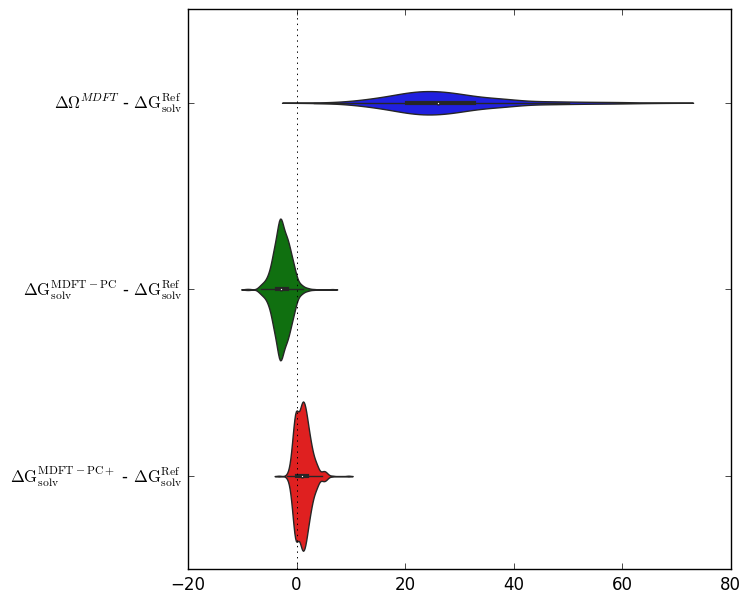
\includegraphics[width=\textwidth]{chapters/BDD/images/freesolv_1/error_distribution_calc_all.png}
         \par\bigskip
         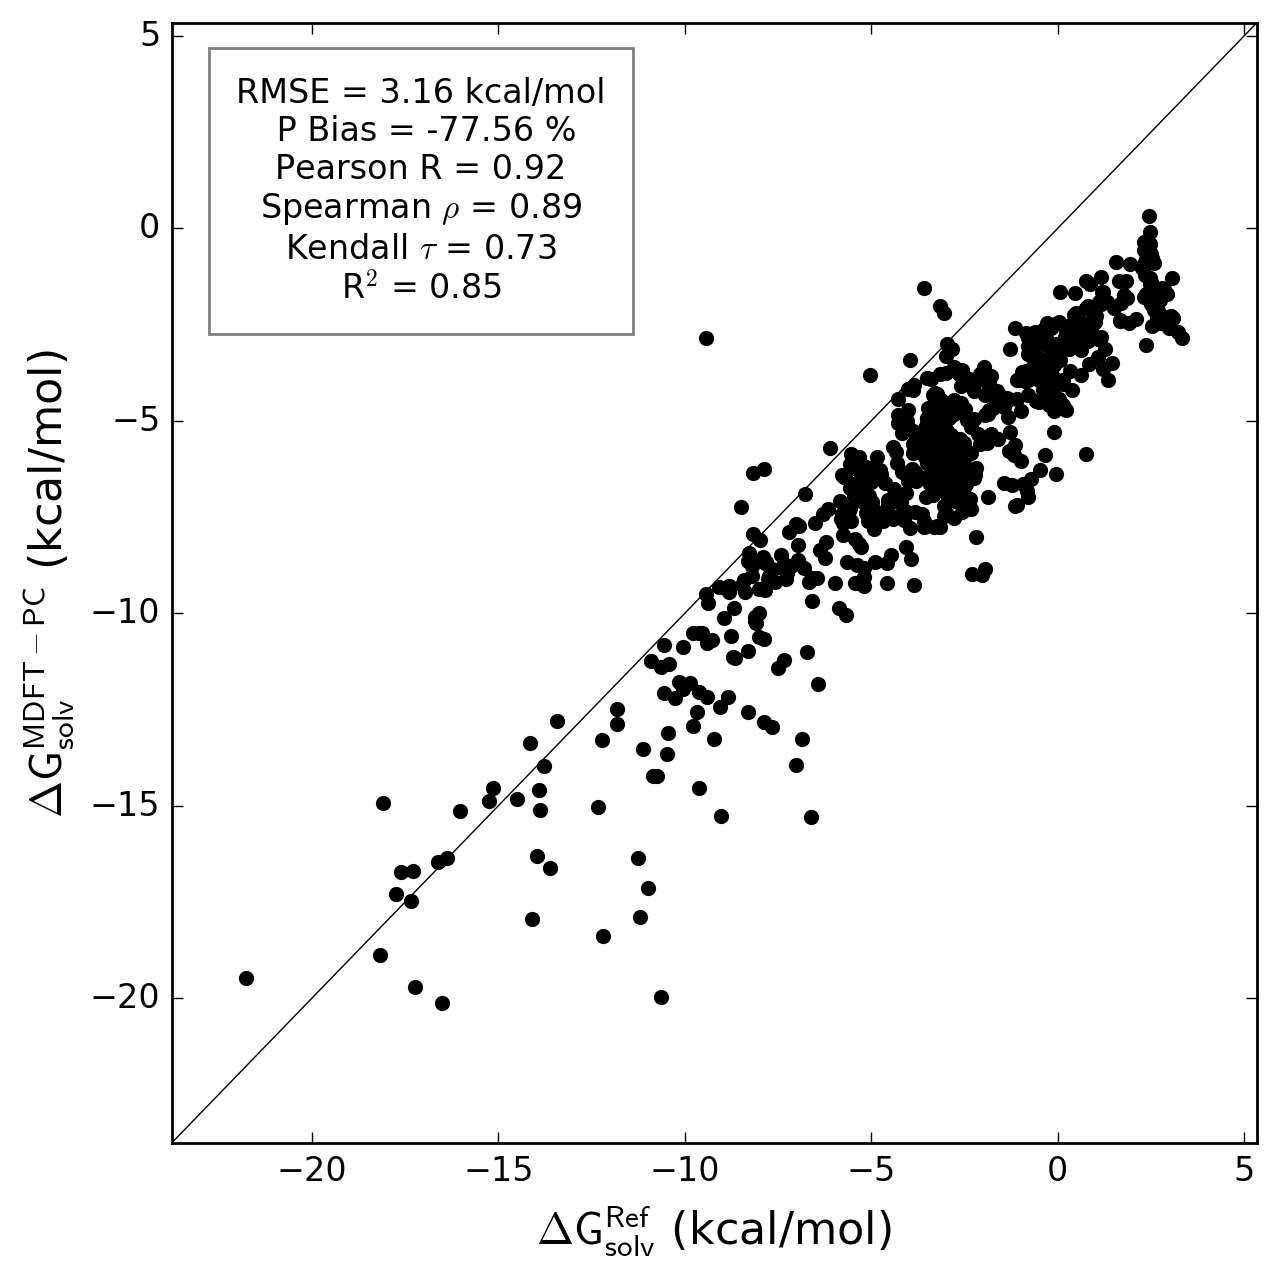
\includegraphics[width=\textwidth]{chapters/BDD/images/freesolv_1/correlation__mdft_energy_pc__vs__calc.png}
   \end{subfigure}
   \hspace{5mm}
   \begin{subfigure}[b]{0.59\textwidth}
         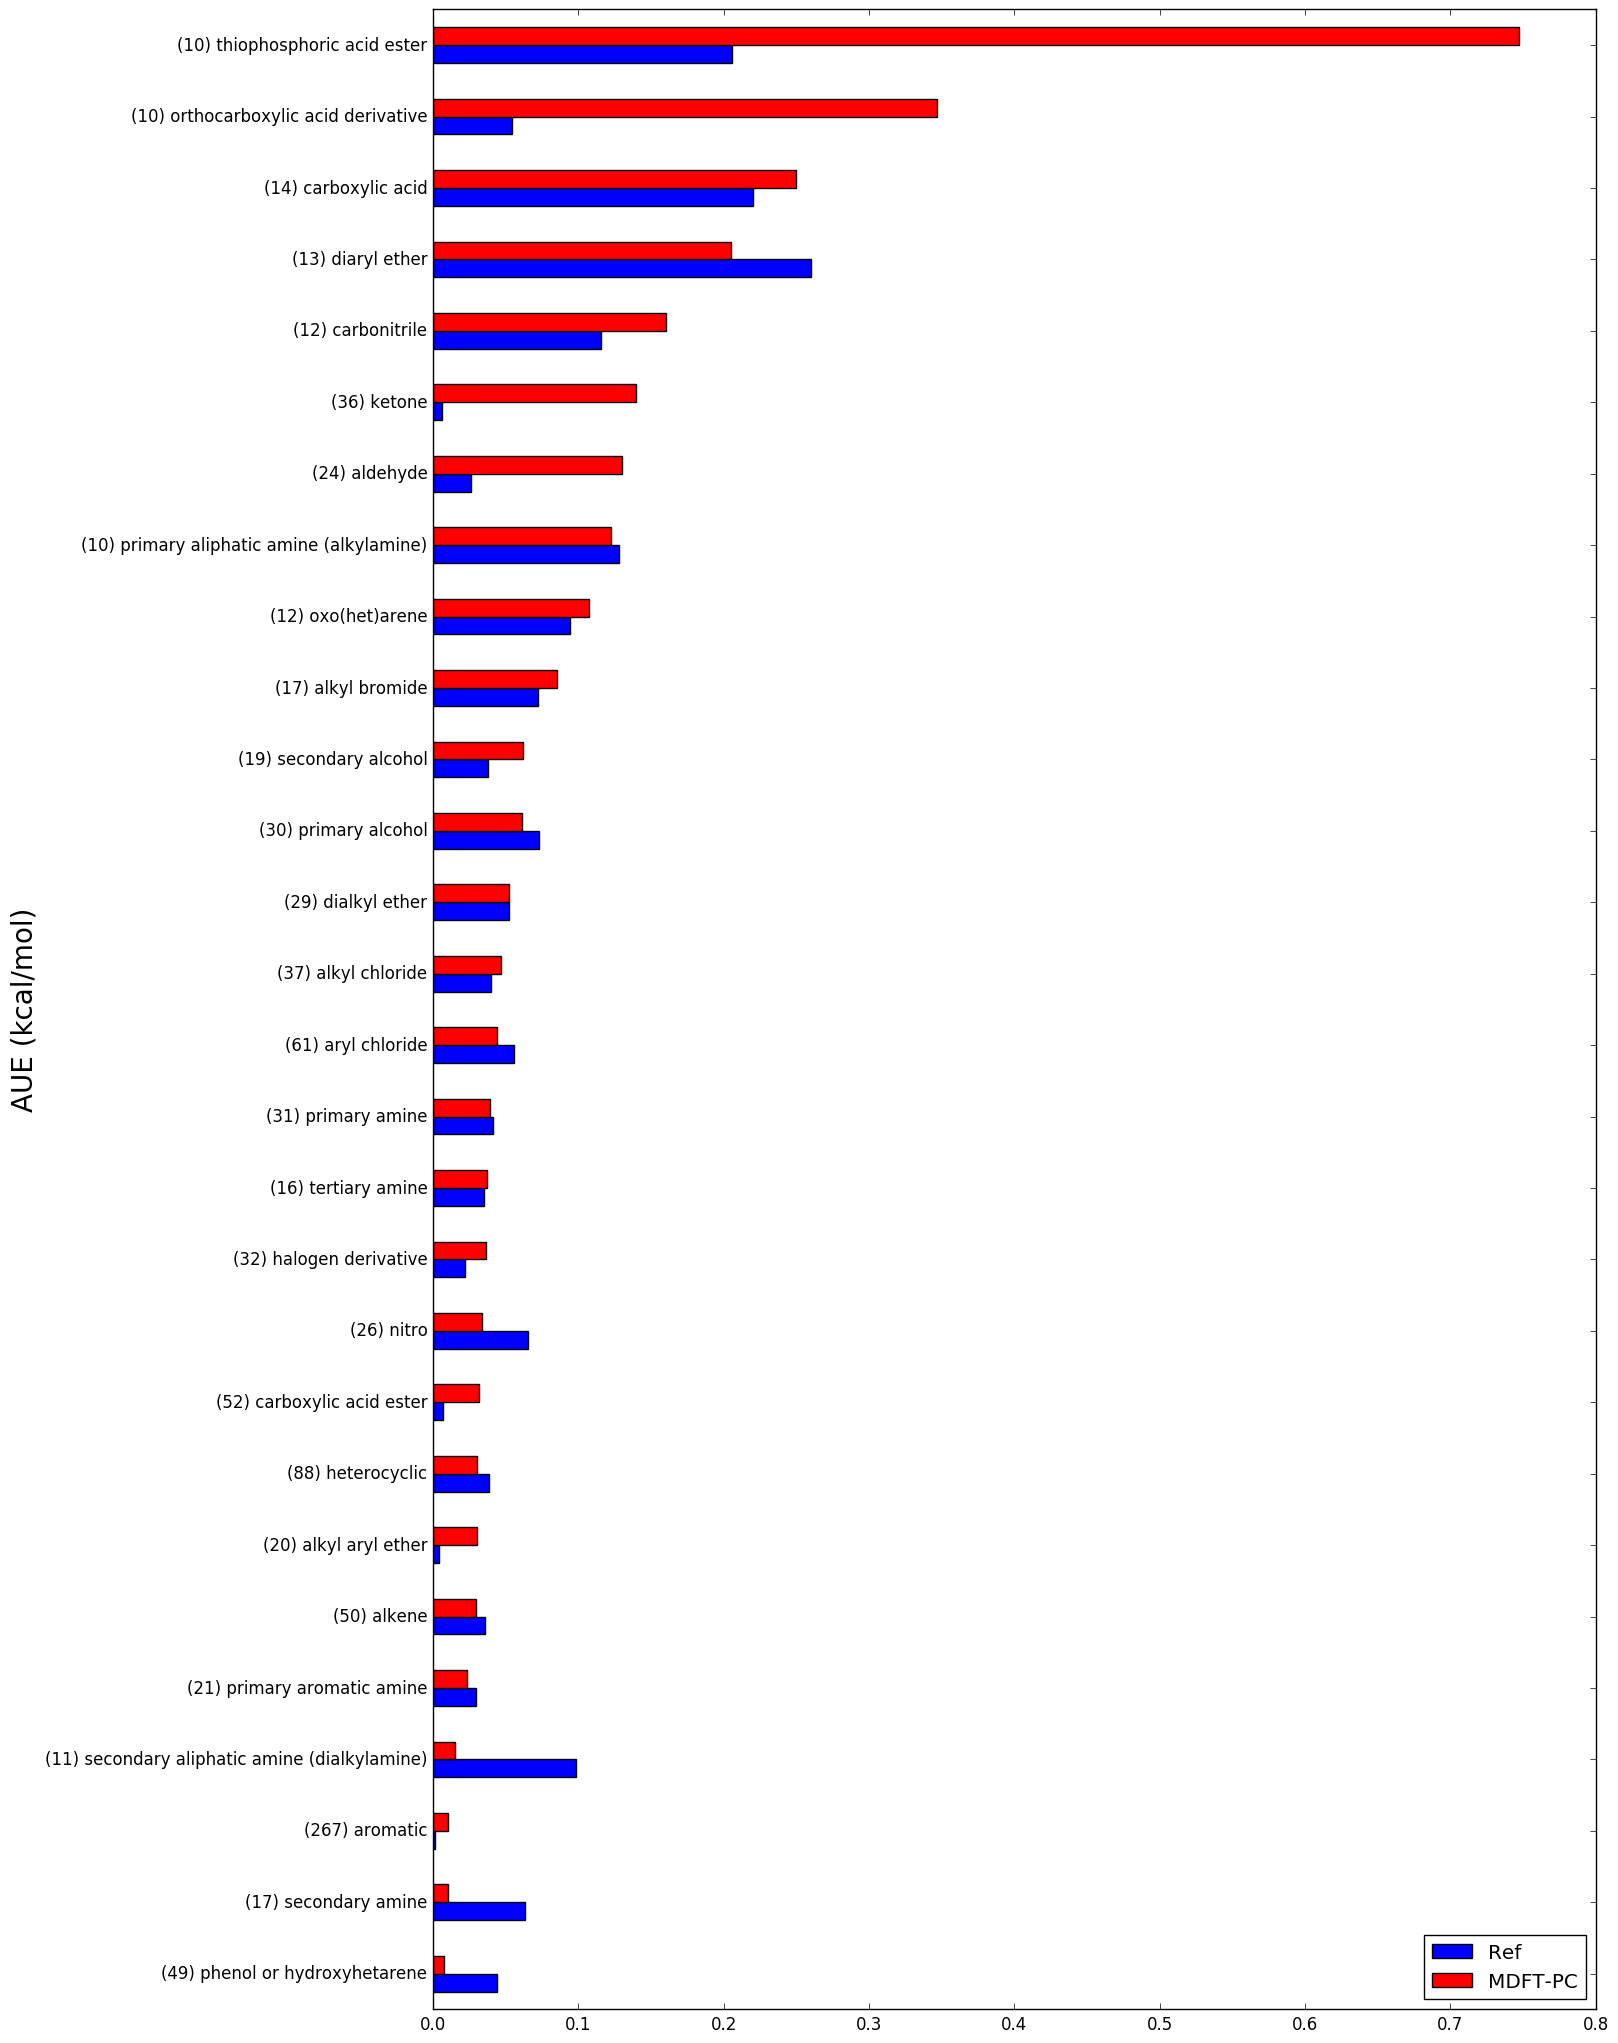
\includegraphics[width=\textwidth]{chapters/BDD/images/freesolv_1/PC_error_by_groups.png}
    \end{subfigure}
  \caption{Exemple d'images d'analyses. En haut à gauche un exemple de violon. En bas à gauche, un exemple de corrélation et à droite un exemple d'analyse par groupe chimique.}
  \label{fig:examples}
\end{figure}


\subsection{La modularité du code}
Un effort tout particulier à été porté afin que le code soit le plus modulable et maintenable possible. 

\subsubsection{Les bases de données}
Aujourd'hui, deux formats de base de données sont implémentées dans ce code. Le format gromacs (fichiers gro et top) qui permet l'étude de la base de données FreeSolv et le format JSON qui permet de créer facilement des chimiothèques. Ces chimiothèques peuvent être soit créées par d'autres codes de références, soit des chimiothèque de références dans le groupe. Le code à été pensé pour qu'il soit facile d'ajouter de nouveaux formats de base de données. Il suffit pour cela uniquement d'implémenter ou de lier le \textit{parser} adapté.

Chaque base de données est ensuite décrites dans un fichier de configuration: lien git ou local, format, valeurs présentes etc..

\subsubsection{Les supercalculateurs}
Actuellement, il est possible de lancer MDFT sur sa propre machine, ou sur le cluster du pôle théorie. nommé "abalone". Nous avons développé ce logiciel de façon à ce qu'il soit très simple d'ajouter un nouvel ordinateur cible. Pour cela, deux fichiers suffisent: un fichier de paramètres en json, ainsi qu'un fichier d'exemple d’exécution.

\subsubsection{Les images d'analyse}
De même, la gestion des images est entièrement externalisée. Un fichier de paramètres regroupe l'ensemble des descripteurs de chaque graphs, comme le type, les valeurs, les labels ou encore l'unité dans lequel il doit apparaître. Les valeurs extraites sont automatiquement converties dans l'unité choisie et affichées en suivant tous ces paramètres. Pour ajouter des nouvelles images, il suffit d'ajouter une nouvelle entrée dans ce fichier de paramètres.

\subsubsection{Les logiciels à étudiés}
Il est pour l'instant possible de lancer uniquement MDFT. Il est cependant relativement simple d'adapter ce code à d'autres logiciels. Un utilisateur peut vouloir se comparer à d'autres méthodes, comme des simulations de dynamique moléculaire ou de Monte Carlo. Il suffit pour cela, d'implémenter la classe nécessaire à l'écriture des fichier d'entrée de cette méthode et d'adapter légèrement le script d’exécution.




\section{Résultats}
\subsection{Les corrections de pressions}\label{sec:corrections_pression}
% Dans un premier temps, nous avons comparé les différentes corrections de pressions \textit{PC} et \textit{PC+}. Pour cela nous avons lancé MDFT dans l'approximation HNC pour $\mathrm{m}_\mathrm{max}$=1 et 3 et nous avons tracé la distribution de l'erreur par rapport aux valeurs expérimentales. Cette distribution est comparée à la distribution obtenue par Dynamique moléculaire. Comme on le voit sur la figure \ref{fig:distrib_error_PC_PCPlus}, \textit{PC+} fournit des meilleurs résultats pour $\mathrm{m}_\mathrm{max}$=1, alors que \textit{PC} devient meilleur pour un $\mathrm{m}_\mathrm{max}$ plus grand.
Pour rappel, l'approximation HNC engendre une forte surestimation de la pression du système dans les conditions standards de pression et température. Sergiievskyi et al. \cite{sergiievskyi_solvation_2015,sergiievskyi_pressure_2015} [REF 2DRISM, CORREENS XXX] ont proposés une correction ad-hoc rigoureuse basée sur la théorie des liquides: la correction \textit{PC} (voir chapitre XXX). Au moment de ce développement, la théorie MDFT n'était pas encore au niveau HNC. Elle correspondrait aujourd'hui à une approximation de HNC avec $\mathrm{m}_\mathrm{max}$=1. Les auteurs ont également proposé une correction empirique, \textit{PC+}, qui améliore considérablement les résultats sans interprétation physique claire. L'étude de base de données nous permet d'étudier l'efficacité de ces deux corrections. Pour cela, nous avons tracé la distribution de l'écart entre les valeurs calculées par MDFT et les valeurs de références calculées par dynamique moléculaire. Ces calculs ont été lancés sans bridge. Nous rappelons au lecteur que le bridge gros grain précédemment développe, corrige la pression du système et ne nécessite aucune correction de pression.

\begin{figure}[H]
   \begin{subfigure}[b]{0.9\textwidth}
       \centering
       \resizebox{\linewidth}{!}{
         \fbox{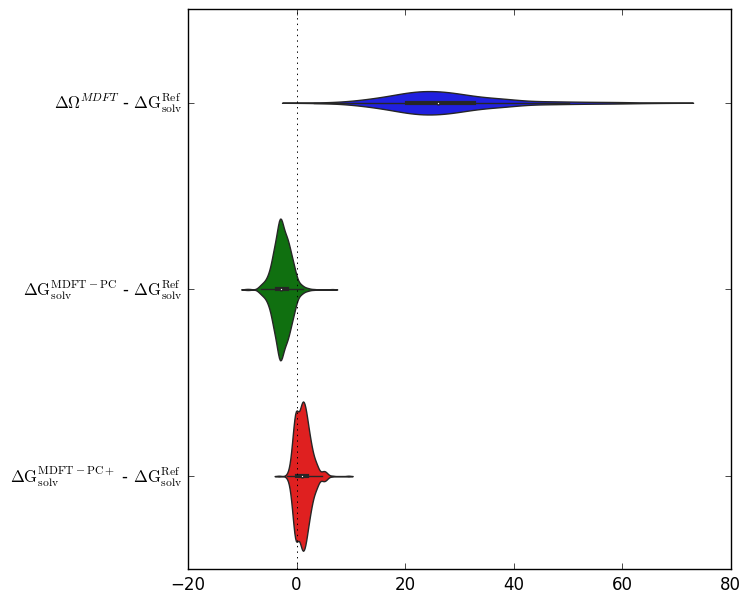
\includegraphics[width=\textwidth]{chapters/BDD/images/freesolv_1/error_distribution_calc_all.png}}
          }
       \caption{$\mathrm{m}_\mathrm{max}$=1}
       \label{fig:distrib_error_PC_PCPlus:mmax1}
    \end{subfigure}
   \begin{subfigure}[b]{0.9\textwidth}
       \centering
       \resizebox{\linewidth}{!}{
         \fbox{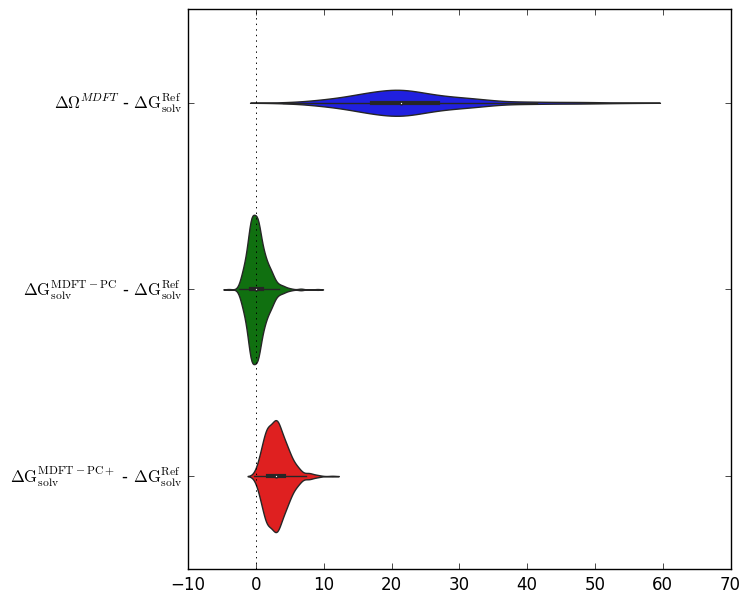
\includegraphics[width=\textwidth]{chapters/BDD/images/freesolv_3/error_distribution_calc_all.png}}
         }
       \caption{$\mathrm{m}_\mathrm{max}$=3}
       \label{fig:distrib_error_PC_PCPlus:mmax3}
    \end{subfigure}
  \caption{Distribution de l'écart entre l'énergie libre de solvatation calculée par MDFT et par dynamique moléculaire sur la base de données freesolv. En bleu, MDFT sans corretion de presion, en vert MDFT avec la correction de pression \textit{PC} et en rouge, MDFT avec la correction de pression \textit{PC+}, pour mmax=1 et 3.}
  \label{fig:distrib_error_PC_PCPlus}
\end{figure}

On voit sur la figure \ref{fig:distrib_error_PC_PCPlus} que la MDFT, sans correction de pression, surestime fortement les énergies libre de solvatation, et ce quelque soit la valeur de $\mathrm{m}_\mathrm{max}$ choisie. Dans tous les cas, les deux corrections de pression \textit{PC} et \textit{PC+} améliore les valeurs et diminuent cet écart à seulement quelques $\mathrm{kJ.mol}^{-1}$. On voit également que pour $\mathrm{m}_\mathrm{max}$=1, la correction \textit{PC} à tendance à sous-estimer les valeurs d'énergies libre de solvatation. Dans ces conditions, mimant au mieux le niveau de théorie disponible au moment du développement de ces corrections, \textit{PC+} améliore bien les résultats. Pour un niveau de théorie supérieur, $\mathrm{m}_\mathrm{max}$=3, la correction \textit{PC} propose des résultats plus précis que la correction \textit{PC+}.

\boitesimple{
Au travers de cette étude, nous avons montré l'efficacité de la correction de pression \textit{PC} quelque soit le niveau de la théorie utilisée. Nous avons également montré que la correction de pression empirique \textit{PC+} permet de corriger simplement les approximations engendrées par l'utilisation d'un mmax=1.
}

\subsection{Le bridge gros grain}
Dans le chapitre précédent, nous avons proposé un nouveau bridge gros grain. Nous avons montré que ce bridge améliore considérablement les structures de solvatation. Afin d'étudier la précision de la prédiction des énergies libres de solvatation, nous avons calculé ces valeurs pour $\mathrm{m}_\mathrm{max}$=1 et $\mathrm{m}_\mathrm{max}$=3 avec et sans le bridge gros grain. Pour chaque jeu de paramètres, nous avons ensuite étudié la corrélation entre les valeurs calculées par MDFT et par dynamique moléculaire.



\begin{sidewaysfigure}
\centering
\begin{figure}[H]
   \begin{subfigure}[b]{0.30\textwidth}
       \centering
       \caption{$\mathrm{m}_\mathrm{max}$=1}
       \resizebox{\linewidth}{!}{
         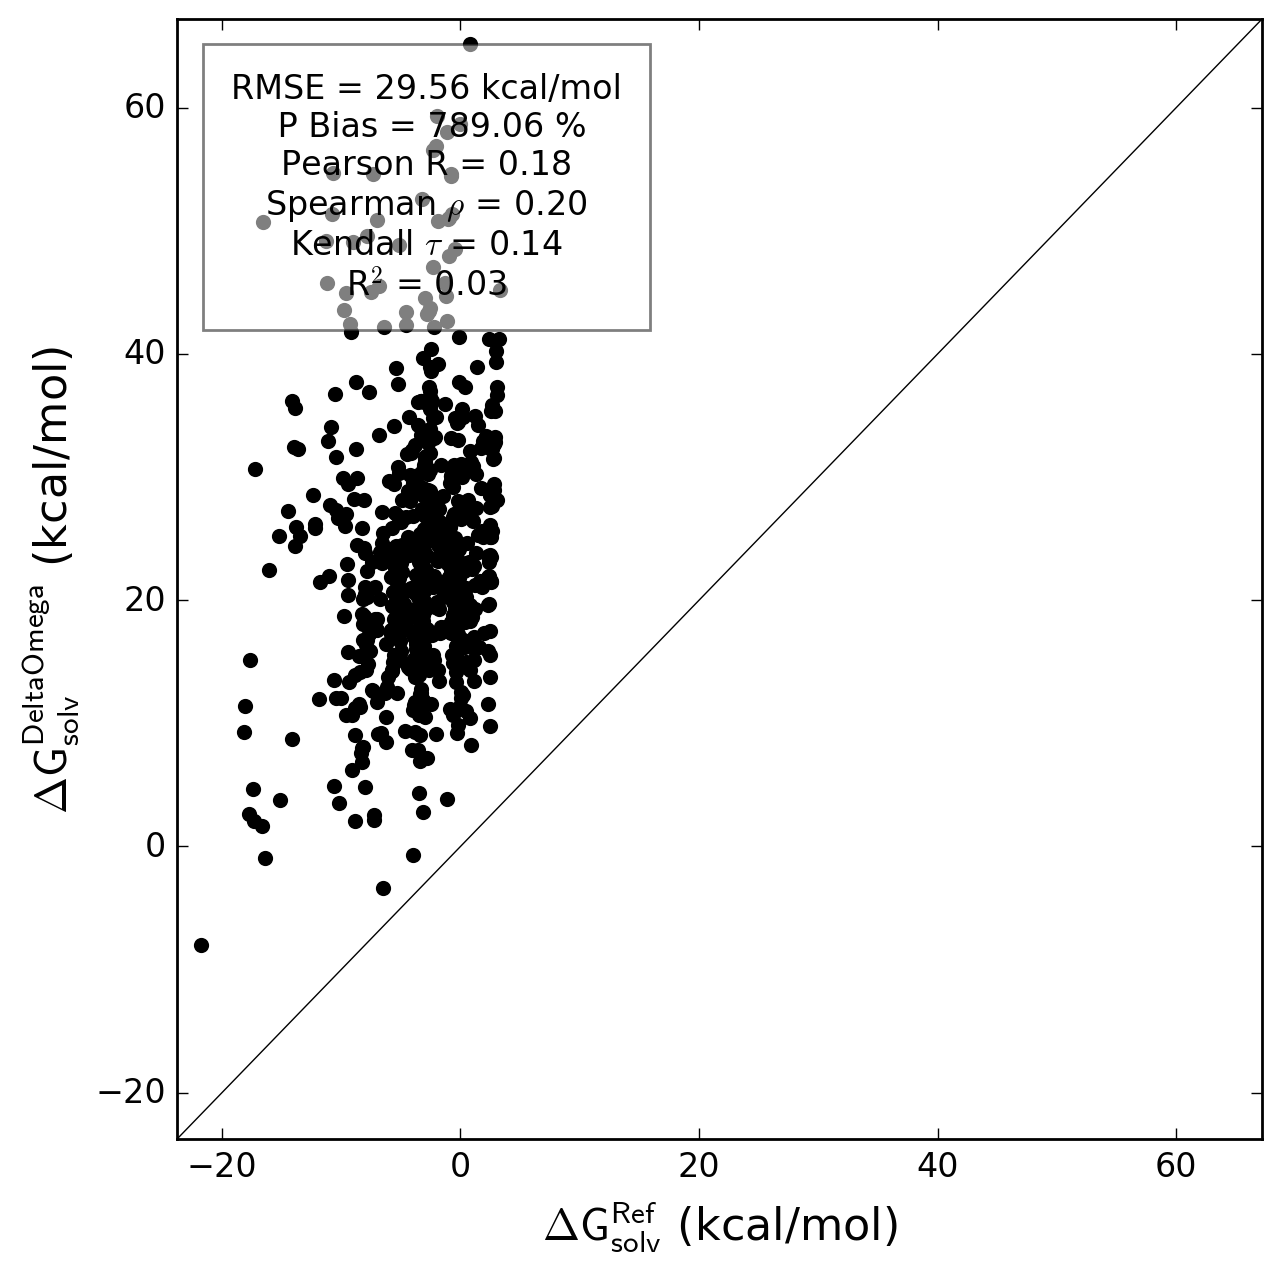
\includegraphics[width=\textwidth]{chapters/BDD/images/freesolv_1/correlation__delta_omega__vs__calc}
          }
       \label{fig:correlation_avec_sans_cgb:mmax1}
    \end{subfigure}    
   \begin{subfigure}[b]{0.30\textwidth}
       \centering
       \caption{$\mathrm{m}_\mathrm{max}$=1,PC}
       \resizebox{\linewidth}{!}{
         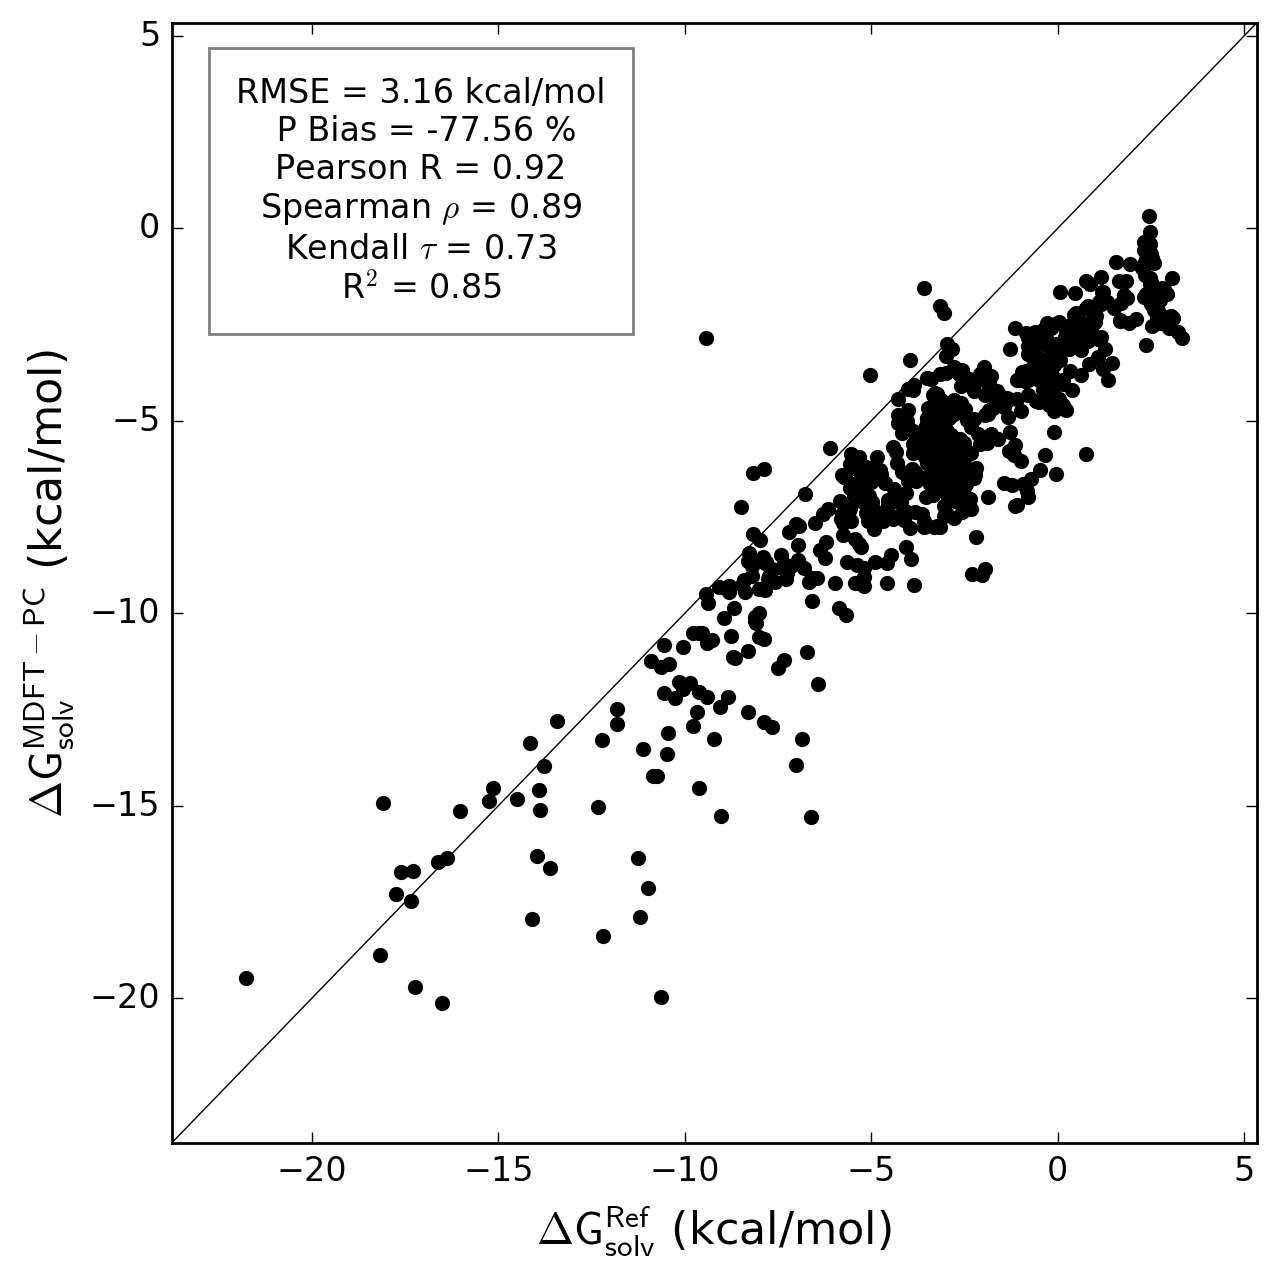
\includegraphics[width=\textwidth]{chapters/BDD/images/freesolv_1/correlation__mdft_energy_pc__vs__calc}
          }
       \label{fig:correlation_avec_sans_cgb:mmax1_pc}
    \end{subfigure}
   \begin{subfigure}[b]{0.30\textwidth}
       \centering
       \caption{$\mathrm{m}_\mathrm{max}$=1,cgb}
       \resizebox{\linewidth}{!}{
         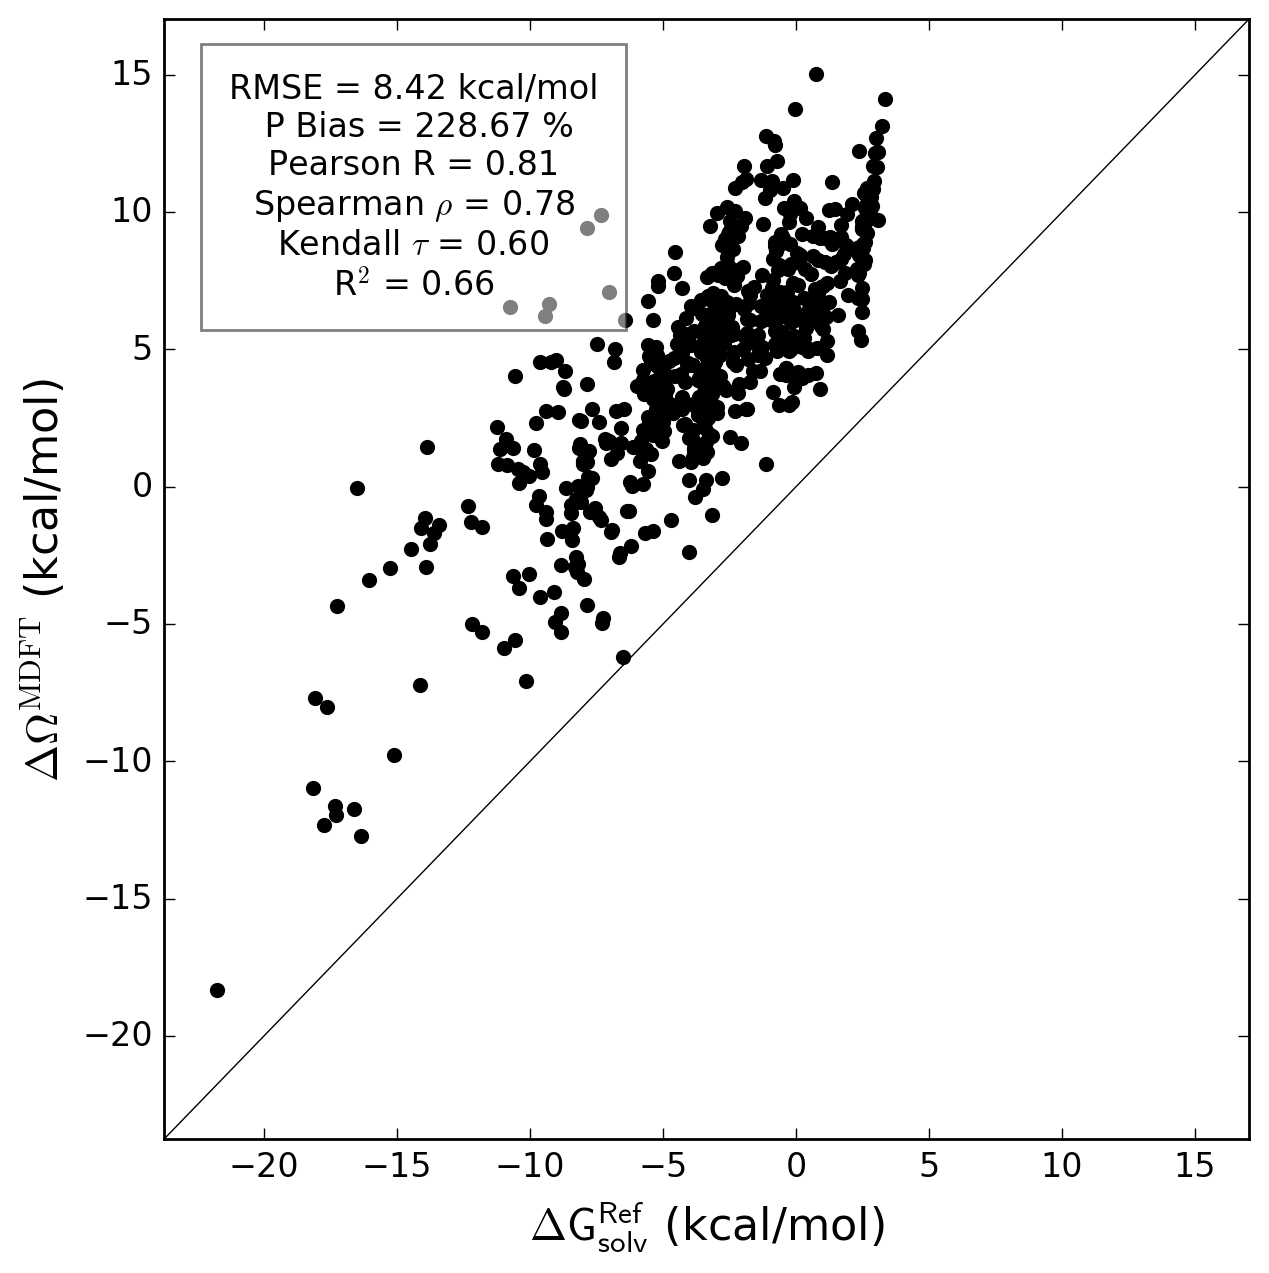
\includegraphics[width=\textwidth]{chapters/BDD/images/freesolv_1_cgb/correlation__delta_omega__vs__calc}
         }
       \label{fig:correlation_avec_sans_cgb:mmax1_cgb}
    \end{subfigure}
    
    
   \begin{subfigure}[b]{0.30\textwidth}
       \centering
       \caption{$\mathrm{m}_\mathrm{max}$=3}
       \resizebox{\linewidth}{!}{
         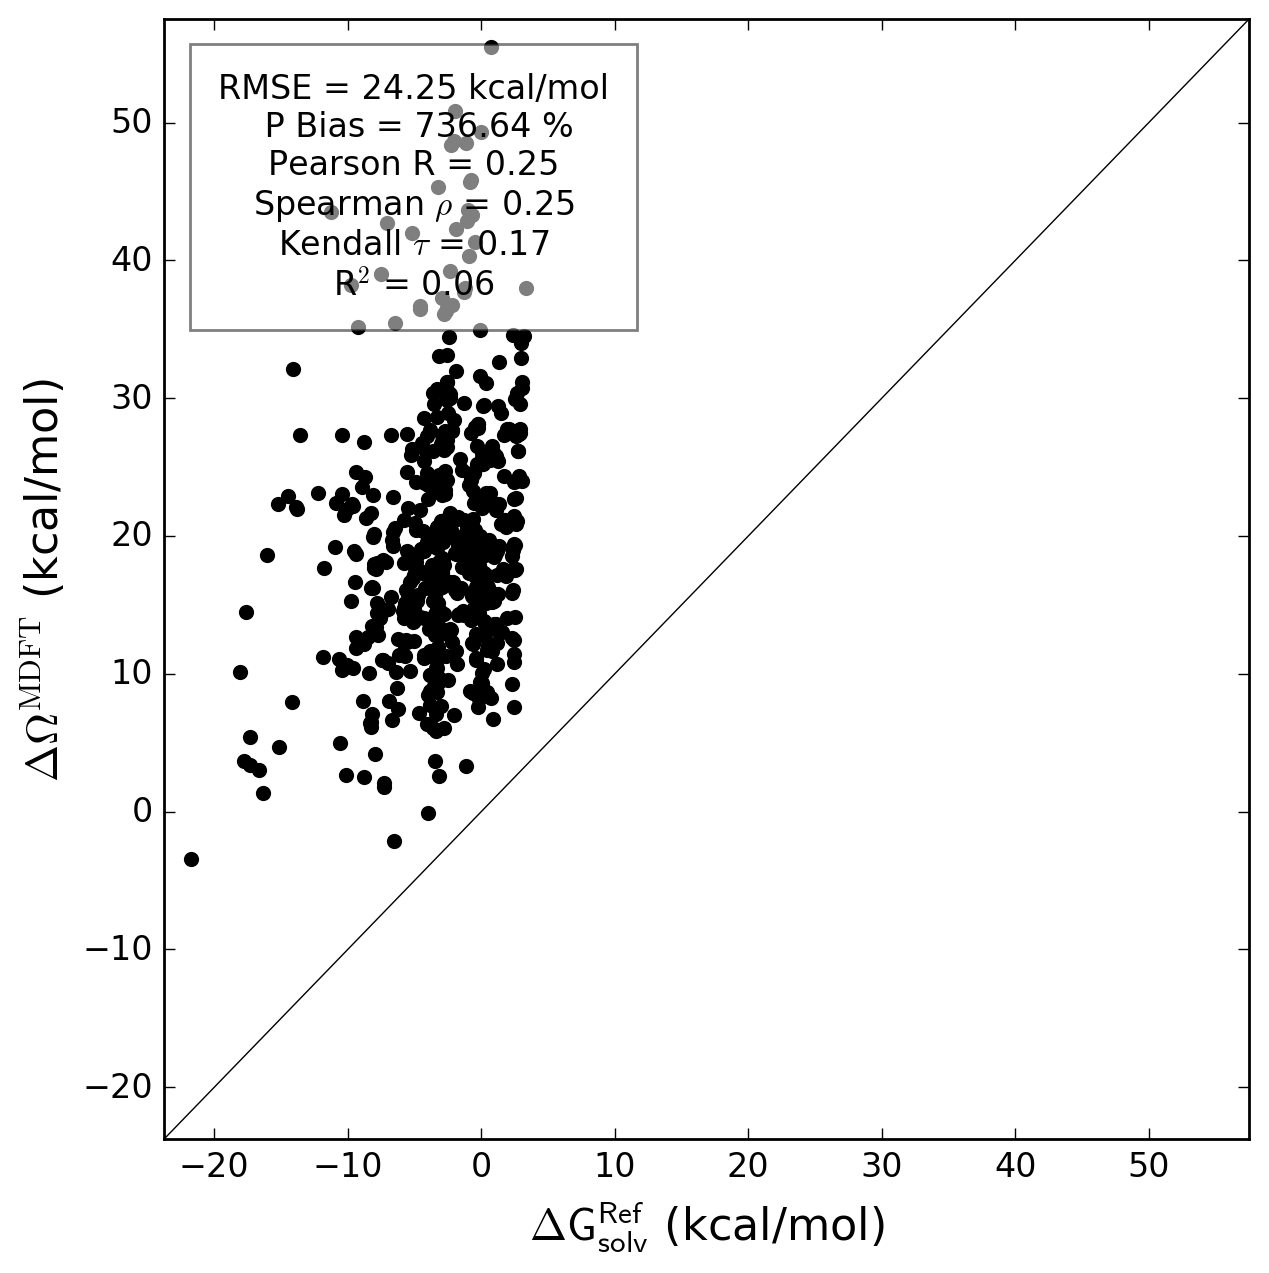
\includegraphics[width=\textwidth]{chapters/BDD/images/freesolv_3/correlation__delta_omega__vs__calc}
          }
       \label{fig:correlation_avec_sans_cgb:mmax3}
    \end{subfigure}    
   \begin{subfigure}[b]{0.30\textwidth}
       \centering
       \caption{$\mathrm{m}_\mathrm{max}$=3,PC}
       \resizebox{\linewidth}{!}{
         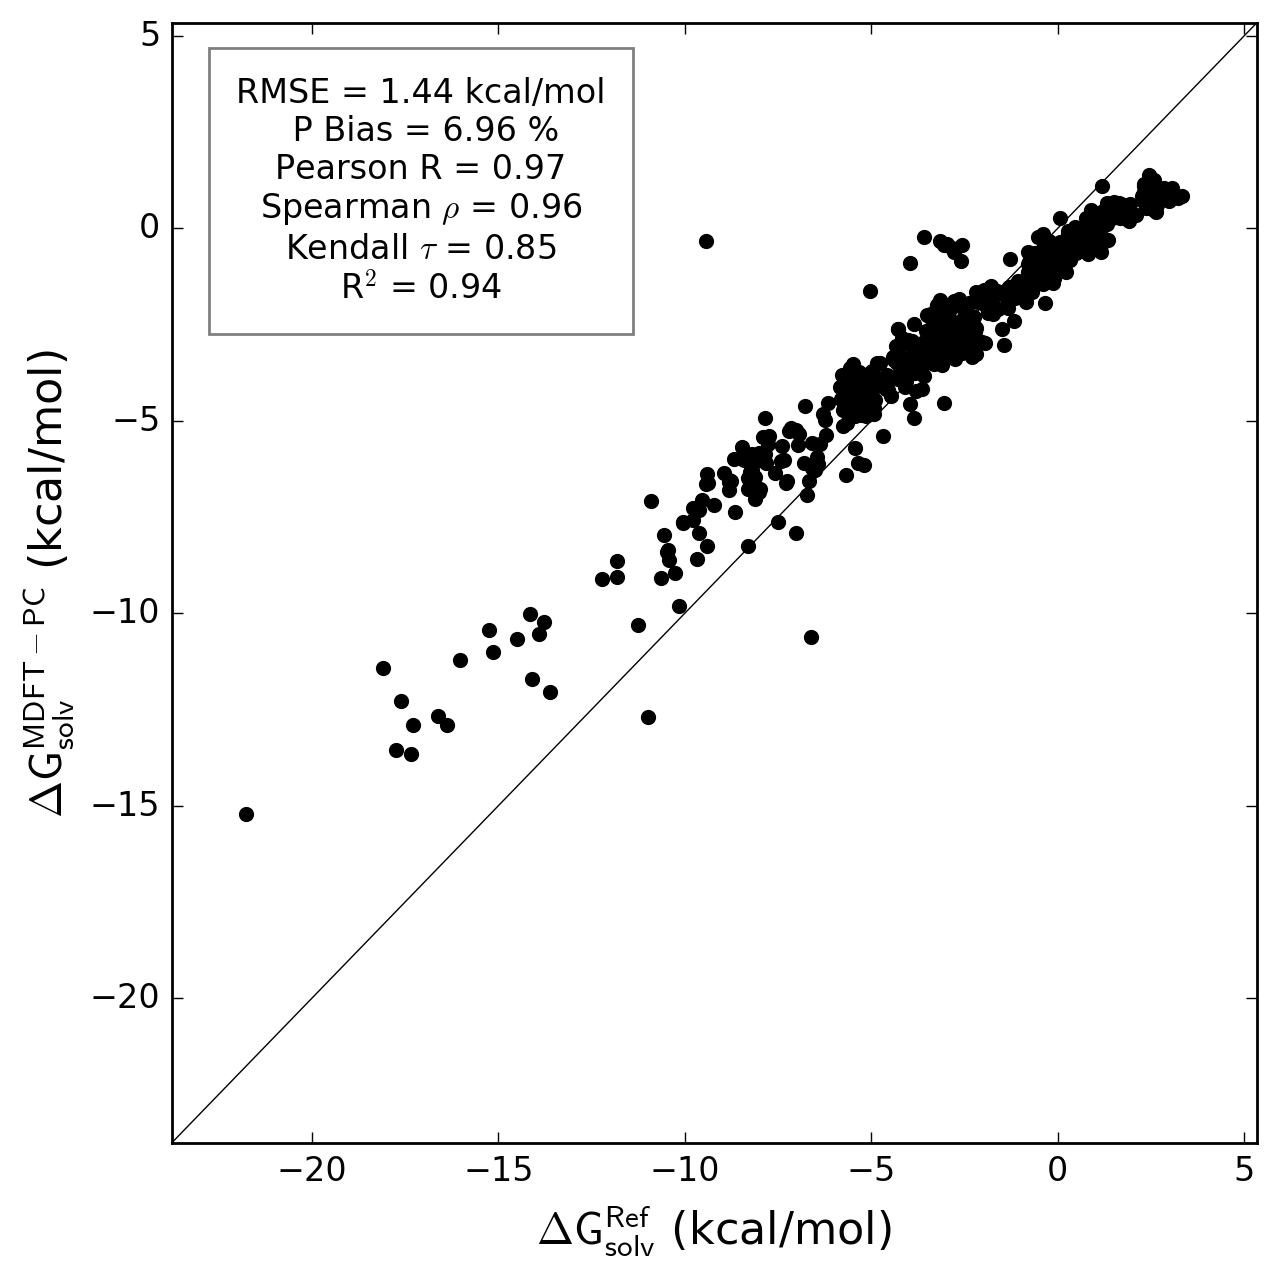
\includegraphics[width=\textwidth]{chapters/BDD/images/freesolv_3/correlation__mdft_energy_pc__vs__calc}
          }
       \label{fig:correlation_avec_sans_cgb:mmax$3_pc}
    \end{subfigure}
   \begin{subfigure}[b]{0.30\textwidth}
       \centering
       \caption{$\mathrm{m}_\mathrm{max}$=3,cgb}
       \resizebox{\linewidth}{!}{
         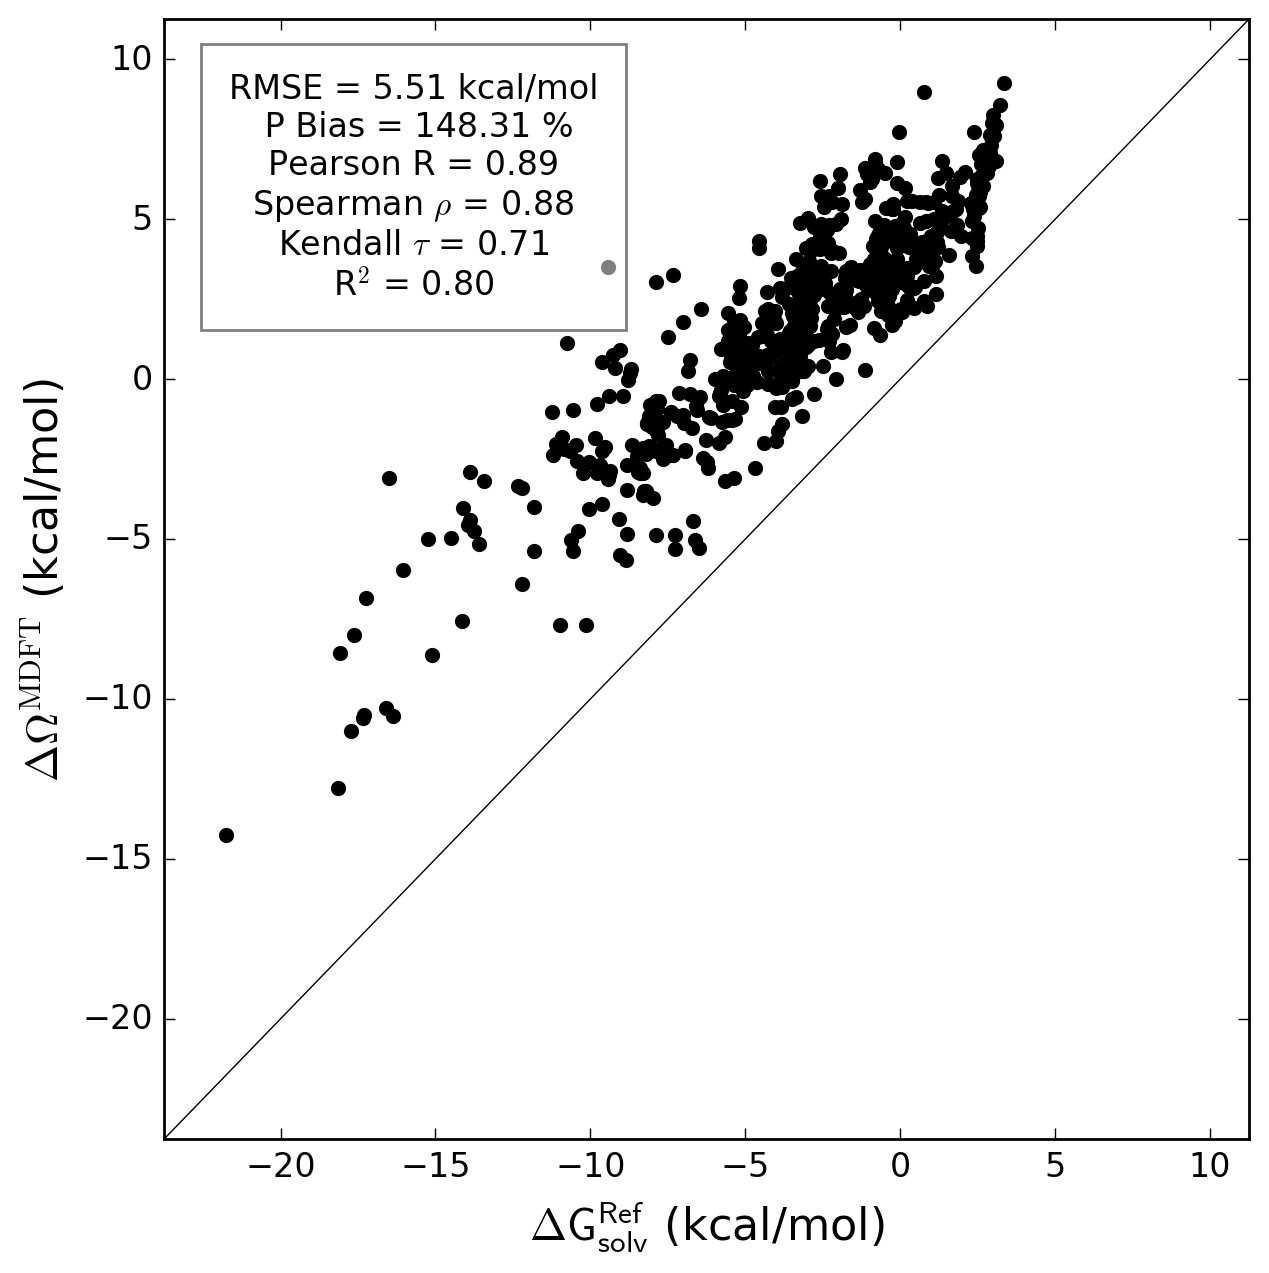
\includegraphics[width=\textwidth]{chapters/BDD/images/freesolv_3_cgb/correlation__delta_omega__vs__calc}
         }
       \label{fig:correlation_avec_sans_cgb:mmax3_cgb}
    \end{subfigure}
    
    
  \caption{Corrélation entre les valeurs d'énergies libres de solvatation calculées par MDFT et par dynamique moléculaire pour les composés de la base de données freesolv. Sur la première ligne $\mathrm{m}_\mathrm{max}$=1, alors que sur la seconde $\mathrm{m}_\mathrm{max}$=3. La première colonne correspond à un calcul MDFT sans correction, la seconde à MDFT avec la correction de pression \textit{PC} et la dernière MDFT avec le bridge gros grain. }
  \label{fig:correlation_avec_sans_cgb}
\end{figure}
\end{sidewaysfigure}


A ce niveau nous disposons de plusieurs possibilités d'améliorations de l'approximation HNC. Soit la pression ad-hoc de pression \textit{PC}, soit le bridge gros grain. Ces deux corrections améliorent fortement les résultats. Comme on peut le voir sur les images \ref{fig:correlation_avec_sans_cgb:mmax1} et \ref{fig:correlation_avec_sans_cgb:mmax3}, il n'existe aucune corrélation entre les valeurs calculées dans l'approximation HNC et les valeurs de références obtenues par dynamique moléculaire. 
Le bridge gros grain ainsi que la correction \textit{PC} améliorent fortement la corrélation de ces données. Avec le bridge, nous obtenons ainsi, pour $\mathrm{m}_\mathrm{max}$=1 $\mathrm{R}^2$=0.66 et pour $\mathrm{m}_\mathrm{max}$=3 $\mathrm{R}^2$=0.80. Avec la correction \textit{PC}, nous obtenons, pour $\mathrm{m}_\mathrm{max}$=1 $\mathrm{R}^2$=0.85 et pour $\mathrm{m}_\mathrm{max}$=3 $\mathrm{R}^2$=0.94. L'ensemble des coefficients de corrélation $\mathrm{R}^2$ est disponible dans le tableau \ref{tab:correlation}.



\begin{table}[H]
  \begin{center}
    \begin{tabular}{ c c }
      \hline & \\[-1em]\hline
       fonctionnelle  & R²  \\
      \hline
       $\mathrm{m}_\mathrm{max}$ 1      & 0.03  \\
       $\mathrm{m}_\mathrm{max}$ 1 PC   & 0.85  \\
       $\mathrm{m}_\mathrm{max}$ 1 cgb  & 0.66  \\
       $\mathrm{m}_\mathrm{max}$ 3      & 0.06  \\
       $\mathrm{m}_\mathrm{max}$ 3 PC   & 0.94  \\
       $\mathrm{m}_\mathrm{max}$ 3 cgb  & 0.80  \\
      \hline & \\[-1em]\hline%
    \end{tabular}
  \end{center}
  \caption{Coefficient de corrélation des énergies libres de solvatation calculées par différentes approximations de MDFT par rapport aux valeurs de référence calculées par dynamique moléculaire. On rappel que plus la valeur est proche et meilleure sera la corrélation.}
  \label{tab:correlation}  
\end{table}



Quelque-soit la valeur du paramètre $\mathrm{m}_\mathrm{max}$, notre bridge gros grain améliore considérablement les résultats par rapport à l'approximation HNC, tout en fournissant des structures de solvatation quasi-parfaites ( voir chapitre XXX ). Ces valeurs d'énergies restent cependant moins précises que celles obtenues avec la correction de pression \textit{PC}.

\boitesimple{
Cette étude nous à permis d'évaluer les différentes corrections dont nous disposons: la correction ad-hoc \textit{PC} et le bridge gros grain. Nous avons ainsi montré que ces deux corrections améliorent fortement la prédiction d'énergies libres de solvatation par rapport à l'approximation HNC seule avec un léger avantage pour la correction de pression \textit{PC}.\\
En fonction des études, nous avons donc le choix entre la correction de pression  \textit{PC}, plus précise au niveau des énergies libres de solvatation, et le bridge gros grain, plus précis en ce qui concerne les profils de solvatation.
}




\subsection{Analyse par groupe chimique}
Pour nous permettre de mieux comprendre les points forts et points faibles de MDFT, nous avons étudié des énergies libres de solvatation en fonction des différents groupes chimiques présents dans la base de données FreeSolv. Afin de ne pas être influencés par la sous représentation de certains groupes chimiques (voir tableau \ref{tab:freeSolvGroupNumbers}), nous ignorons dans ce chapitre les résultats obtenus pour des groupes étant composés de moins de 10 molécules. Une représentation 2D de ces groupes est disponible en figure \ref{fig:groupes_chimiques}. Dans un premier temps nous avons calculée et affichée l'erreur relative moyenne pour chaque groupe avec MDFT et la correction de pression \textit{PC} et avec MDFT et le bridge gros grain.

Nous rappelons au lecteur que les calculs MDFT et dynamique moléculaire utilisent le même champs de force soit GAFF couplé à AM1-BCC pour les charges. Il existe cependant quelques différences notables. La première est le modèle d'eau. En effet MDFT utilise le modèle SPC/E alors les calculs en dynamique moléculaire utilisent eux le modèle TIP3P. De plus, la dynamique moléculaire est effectuée sur des molécules flexibles ce qui n'est pour l'instant pas le cas de MDFT. 

Si le champs de force et la théorie était idéaux, les erreurs moyennes pour chaque groupe et chaque méthode devraient être nulles. La dynamique moléculaire est une méthode considérée comme exacte. Pour un groupe donné, si l'erreur moyenne calculée par dynamique moléculaire s'écarte de zéro, cela signifie donc que le champs de force n'est pas optimal pour le calcul d'énergies libres de solvatation de molécules dans cette zone de l'espace chimique. Au contraire, un écart entre la dynamique moléculaire et la MDFT indique que la théorie de la MDFT n'est pas optimisée pour le groupe chimique en question. Ainsi, si pour un groupe donné, la MDFT est plus précise que la dynamique moléculaire, ces résultats seraient obtenus par chance mais traduiraient en réalité un défaut de notre théorie. 

C'est dans le but de reproduire les énergies libre de solvatations expérimentales, que Sohvi Luukkonen, développe un bridge \textit{machine learning}. Il permet de corriger à la fois les approximations de la MDFT et du champs de force (résultats non présentés dans ce rapport).

\begin{figure}[H]
  \centering
  \resizebox{\linewidth}{!}{
  	\fbox{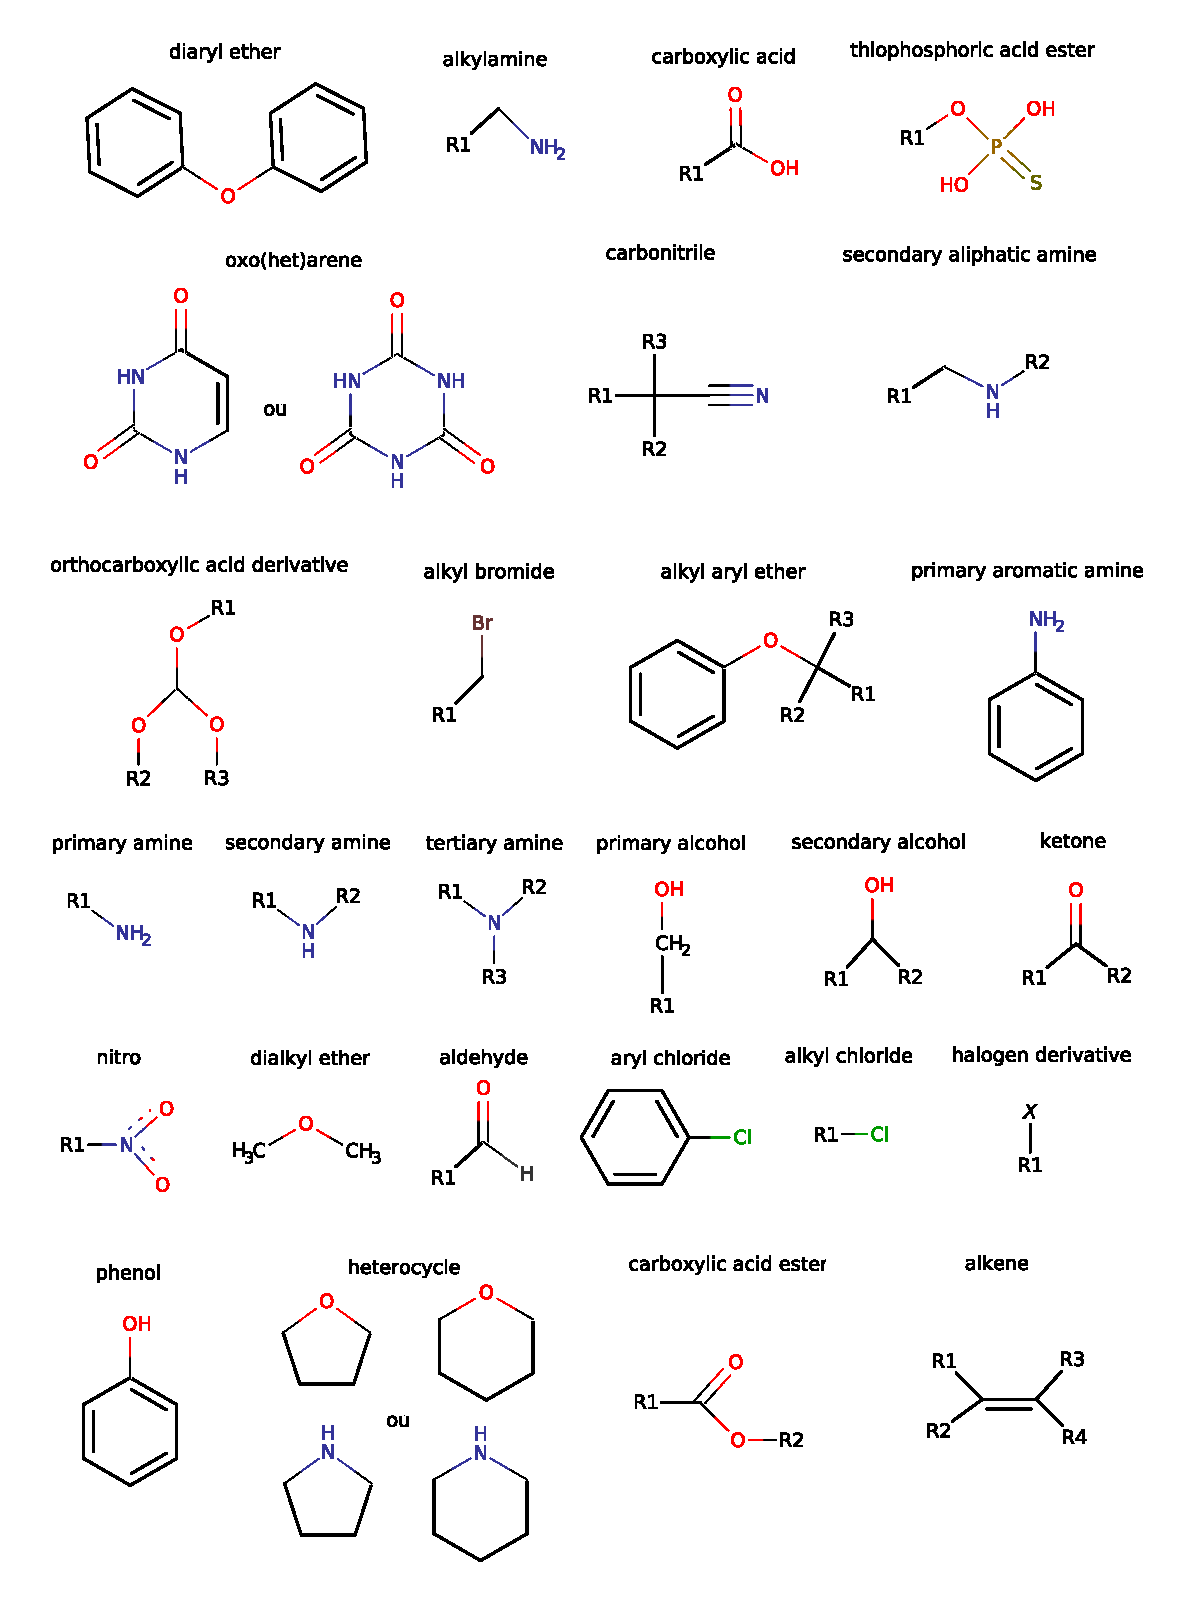
\includegraphics[width=\textwidth]{chapters/BDD/images/groups/groupes_chimiques.eps}}
  }
  \caption{Représentation en 2 dimensions des groupes chimiques étudiés dans ce chapitre. \protect\footnotemark}
  \label{fig:groupes_chimiques}
\end{figure}
\footnotetext{Image réalisée avec le logiciel MarvinSketch 17.17.0 , 2017, ChemAxon (\url{http://www.chemaxon.com}).}

\begin{figure}[H]
  \centering
  \resizebox{\linewidth}{!}{
  	\fbox{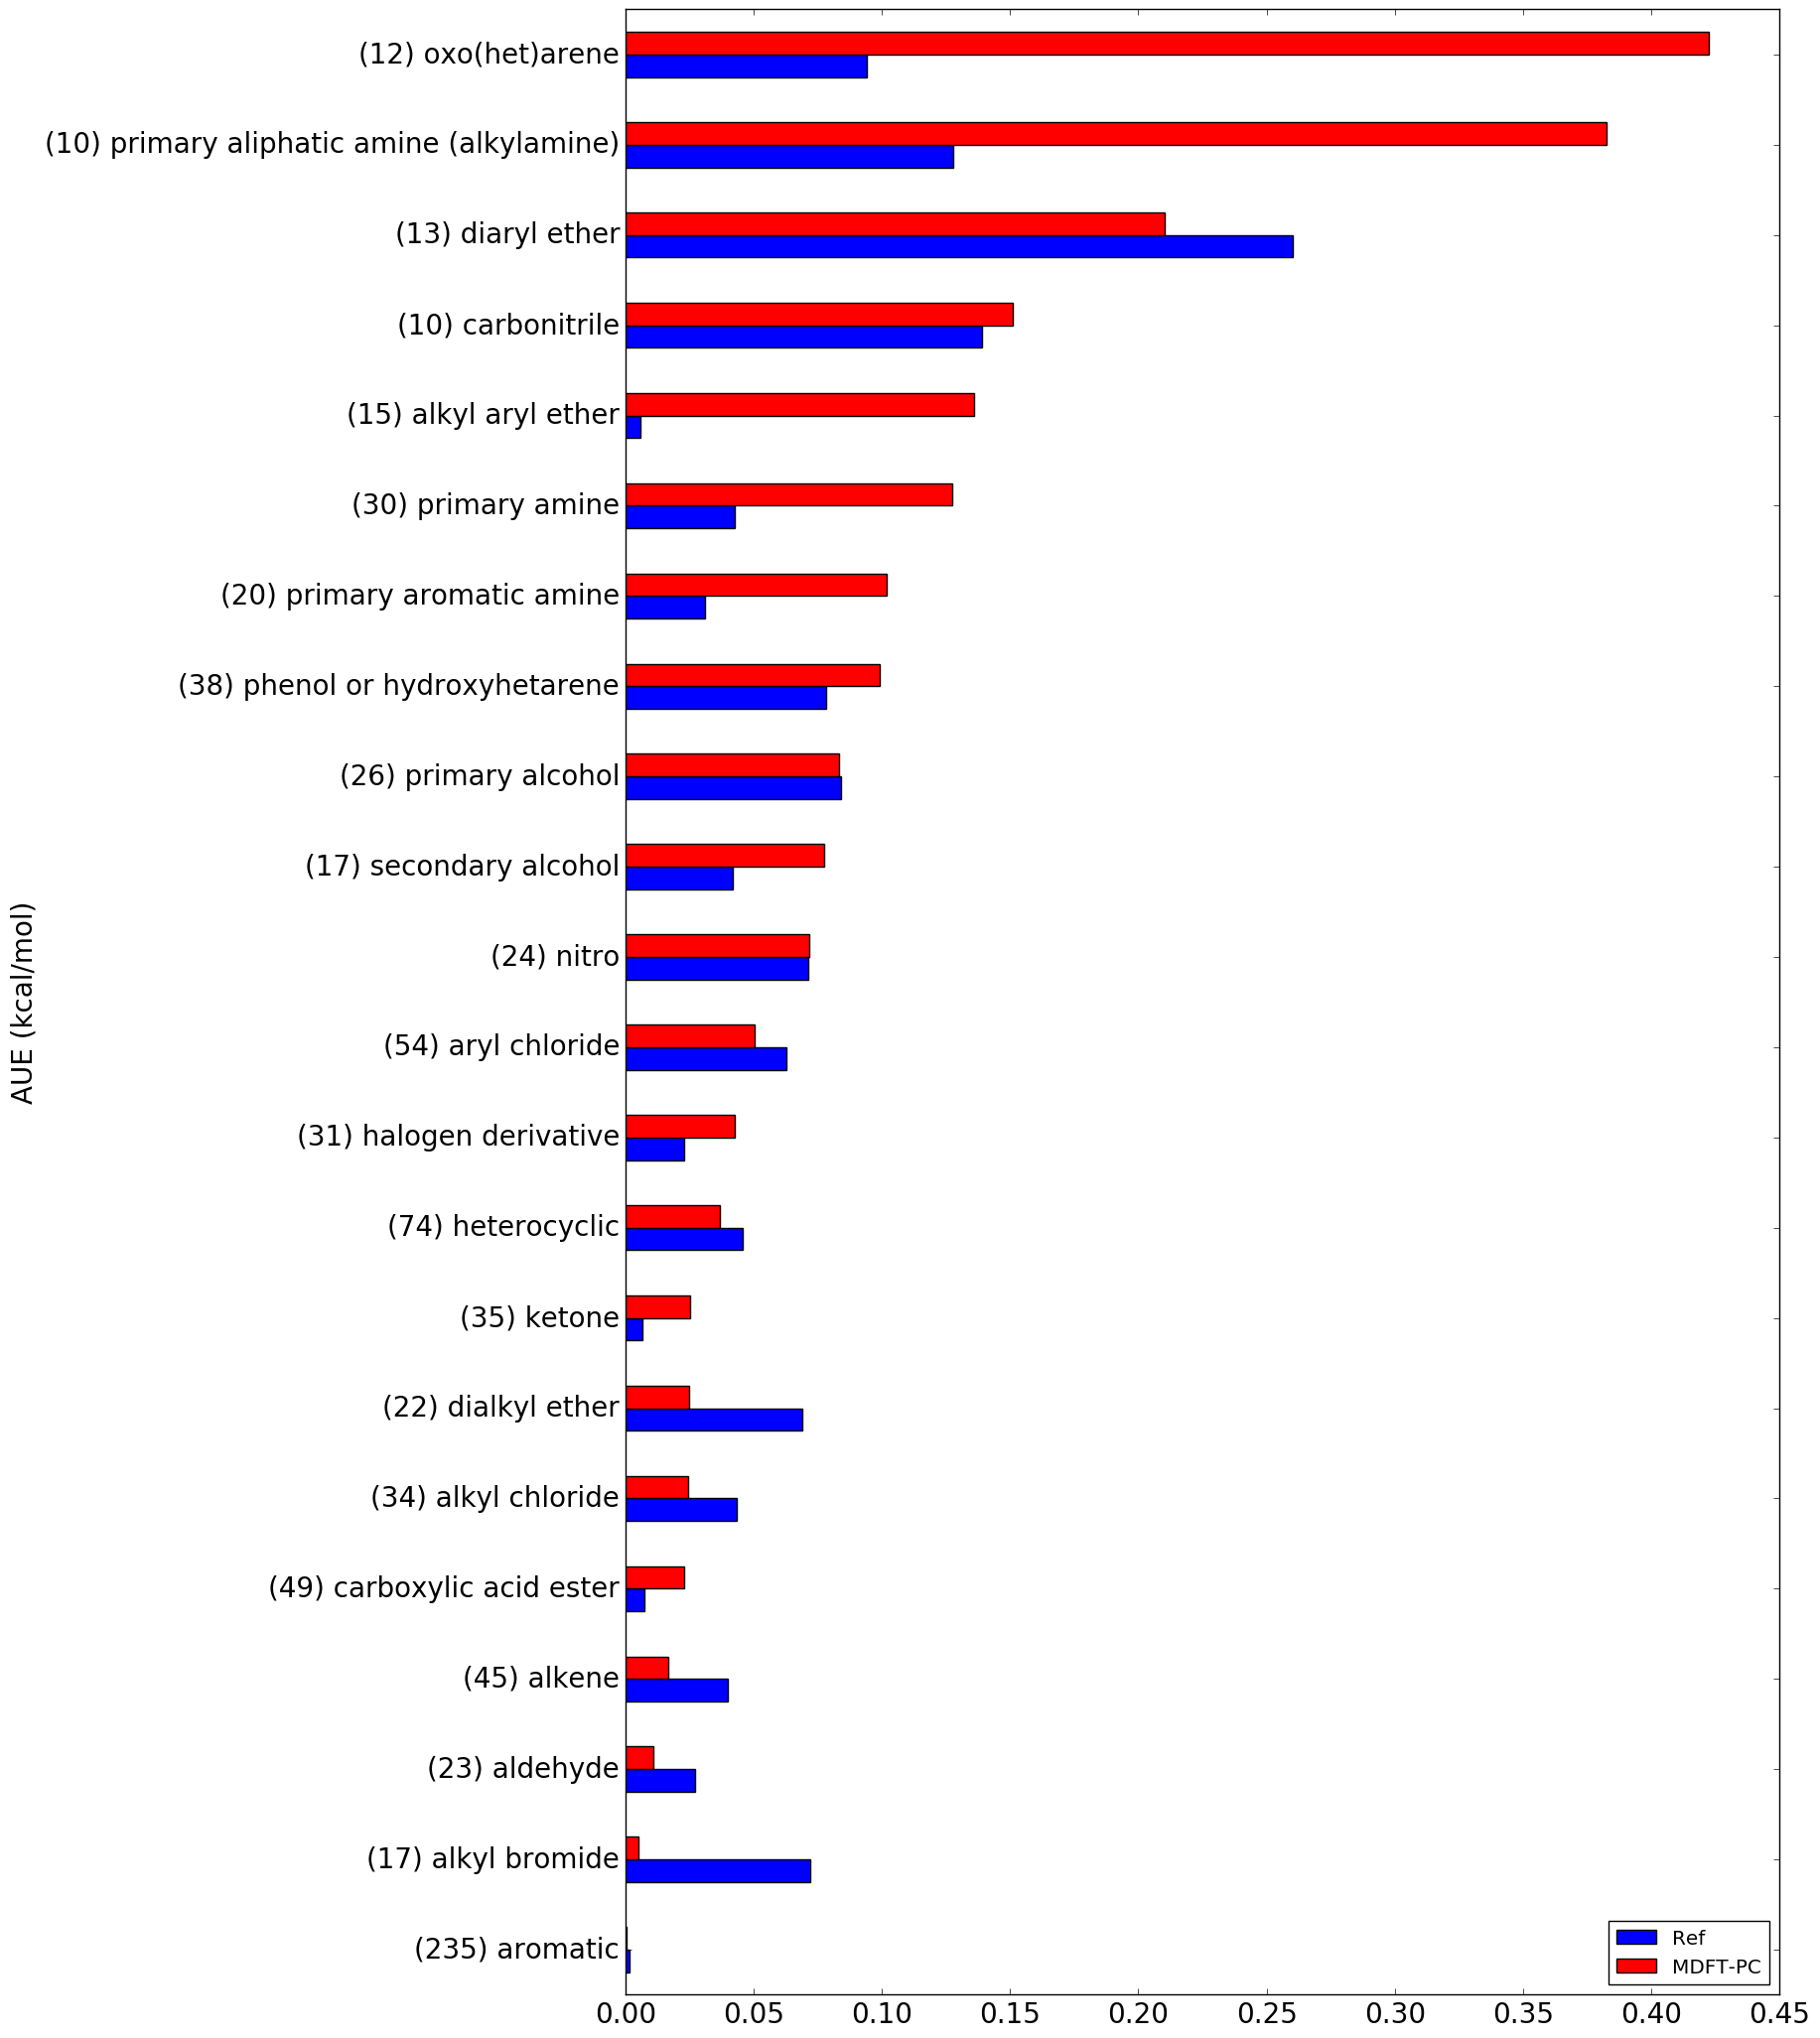
\includegraphics[width=\textwidth]{chapters/BDD/images/freesolv_3/PC_error_by_groups}}
  }
  \caption{Erreur absolue moyenne calculée pour chaque groupe chimique, par rapport aux valeurs expérimentales. En bleu, les résultats de dynamique moléculaire et en vert ceux de MDFT pour $\mathrm{m}_\mathrm{max}$=3 avec la correction de pression \textit{PC}. Nous n'affichons ici que les groupes comportant 10 molécules ou plus.}
  \label{fig:AUE:mmax3}
\end{figure}



\begin{figure}[H]
  \centering
  \resizebox{\linewidth}{!}{
  	\fbox{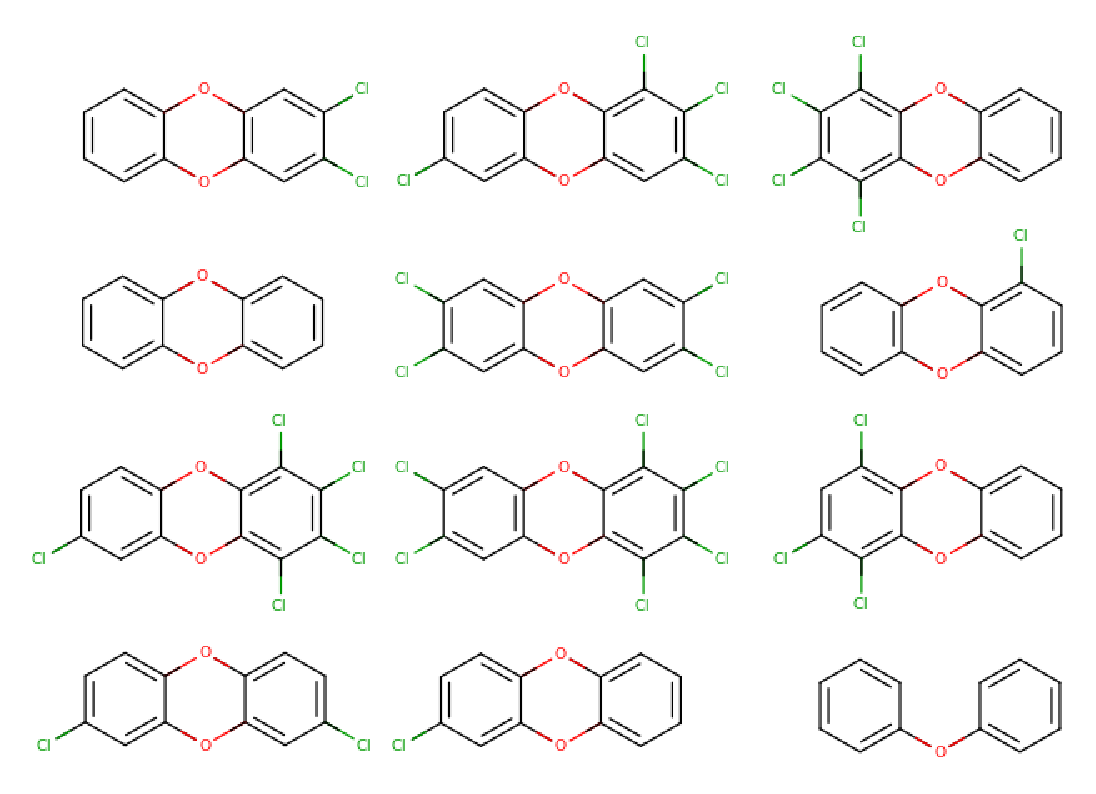
\includegraphics[width=\textwidth]{chapters/BDD/images/groups/diaryl_ether.eps}}
  }
  \caption{Représentation en 2 dimensions des molécules composant le groupe des diaryl ethers.}
  \label{fig:diaryl_ether}
\end{figure}

Dans un premier temps, on voit que la dynamique moléculaire et donc le champ de force est moins précis pour les diaryl ether, les alkylamines ou encore les carbonitriles. Ces résultats sont cependant à prendre avec précautions car ces groupes peuvent être peuplés par des molécules similaires comme c'est le cas pour les diaryl ether (voir figure \ref{fig:diaryl_ether}). En effet, la base de données Freesolv est issue de la littérature et il est fréquent que des molécules soient étudiées par séries. Dans le cas des diaryle ether, cette série de molécules, correspond à la fraction d'une série plus importante qui à été utilisée lors du challenge SAMPL3\cite{Geballe_sampl_2012}. Ces déséquilibres n'ont cependant aucun impacte sur la comparaison de la dynamique moléculaire et de la MDFT car le biais est identique dans les deux cas.

Cette étude nous permet également de confirmer deux points faibles de MDFT: l'hydrophobicité (voir chapitre XXX) et les charges partielles[REF LU XXX]. En effet, les différences les plus importantes entre les deux méthodes sont obtenues pour les oxo(het)arenes (charges partielles), les amines primaires aliphatiques(charges partielles), les alkyl aryl éthers(charges partielles, hydrophobe), les amines primaires(charges partielles) et les amines primaires aromatiques (charges partielles, hydrophobe). 



\begin{figure}[H]
  \centering
  \resizebox{\linewidth}{!}{
         \fbox{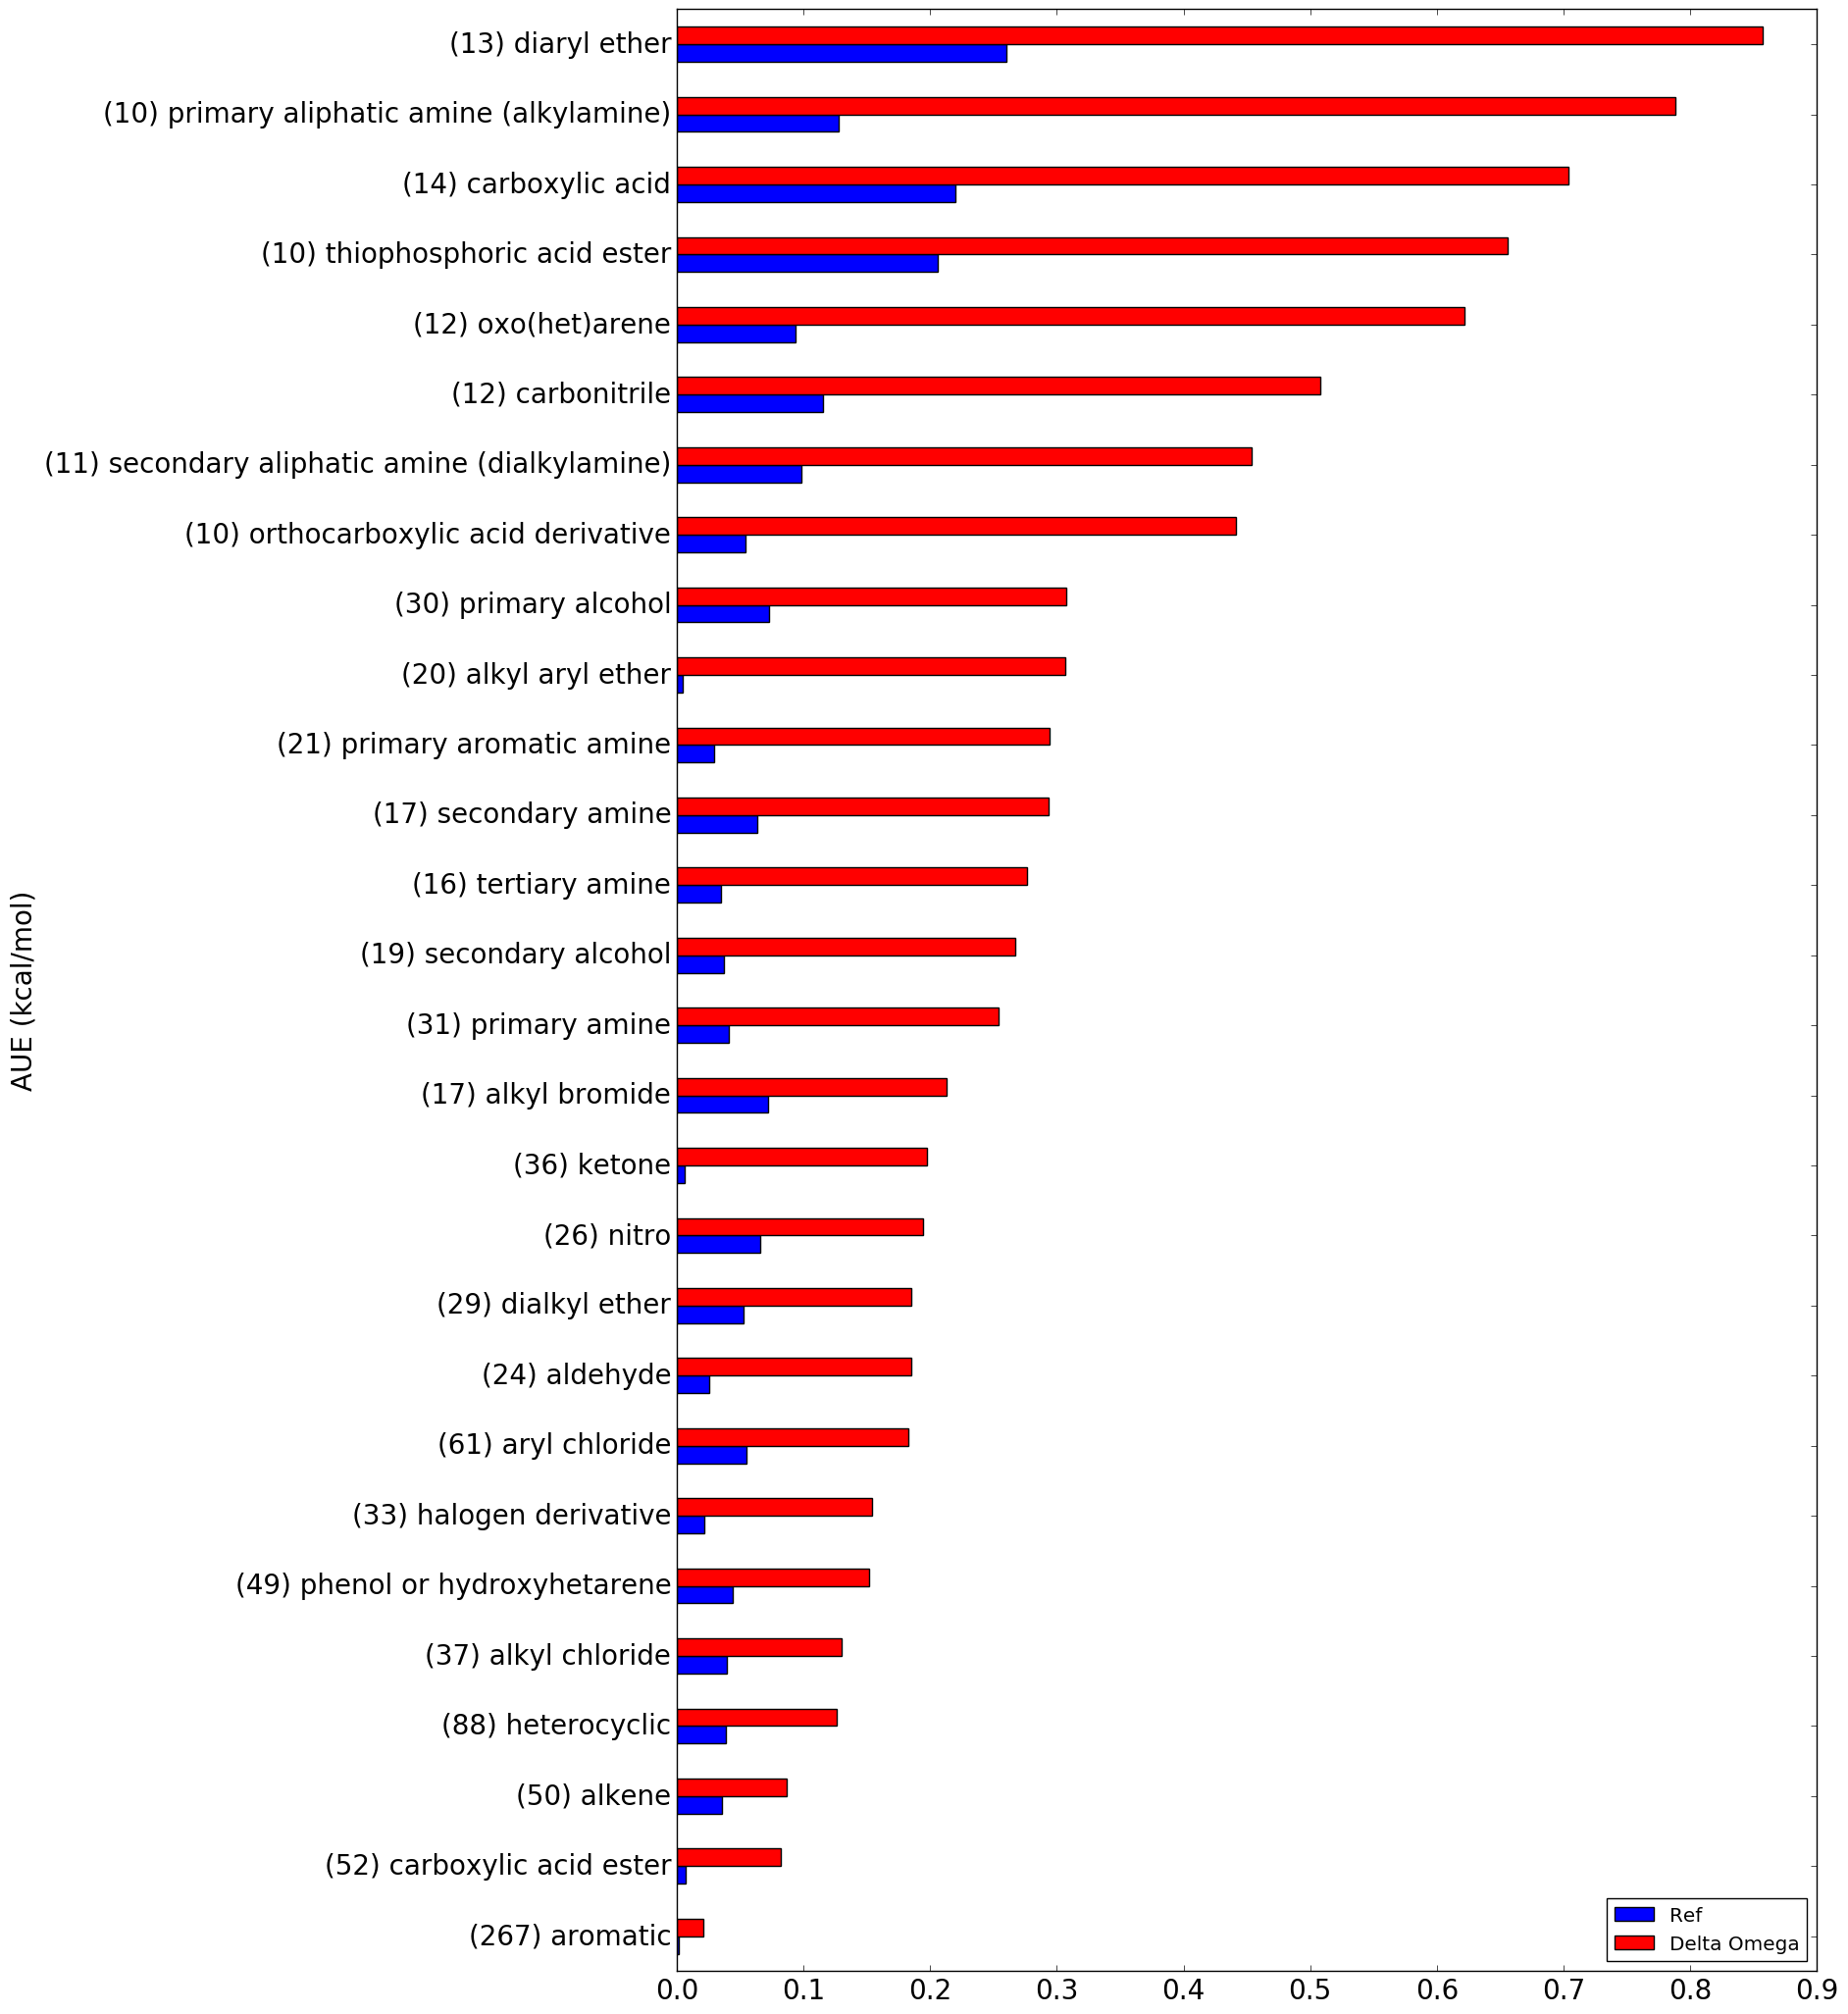
\includegraphics[width=\textwidth]{chapters/BDD/images/freesolv_3_cgb/HNC_error_by_groups}}
  }
  \caption{Erreur absolue moyenne calculée pour chaque groupe chimique, par rapport aux valeurs expérimentales. En bleu, les résultats de dynamique moléculaire et en vert ceux de MDFT pour $\mathrm{m}_\mathrm{max}$=3 avec le bridge gros grain. Nous n'affichons ici que les groupes comportant 10 molécules ou plus.}
  \label{fig:AUE:mmax3_cgb}
\end{figure}



Enfin, on voit que MDFT avec le bridge gros grain, nous donne globalement des erreurs plus importantes avec une erreur maximale autour de 0.85 kcal.mol$^{-1}$ contre 0.43 kcal.mol$^{-1}$ pour MDFT avec la correction de pression \textit{PC}. Ces résultats confirment ceux précédemment obtenus dans le paragraphe \ref{sec:corrections_pression}. 






\boitesimple{
Dans cette partie, nous avons mis en évidence des groupes chimiques qui exacerbent les faiblesses de MDFT. Ces groupes sont principalement hydrophobes ou contiennent des charges partielles importantes. L'hydrophobocité ayant été traitée dans le chapitre précédent, nous étudions dans la suite de ce chapitre une base de données d'ions afin de mieux comprendre l'impacte des charges sur MDFT.
}





\section{Les ions}
En plus de l'analyse de base de données officielles comme FreeSolv, ce logiciel nous permet d'étudier simplement et efficacement un ensemble de molécules d’intérêts. Nous nous en sommes donc servit afin d'étudier l'impacte de la charge sur les résultats de MDFT. Notre jeux de données est composé de 4 cations: Li$^+$, Na$^+$, K$^+$, Cs$^+$ et de 4 anions F$^-$, Cl$^-$, Br$^-$, I$^-$.
Dans un premier temps nous avons comparé les énergies libres de solvatations calculées par MDFT et par dynamique moléculaire\cite{Horinek_rational_2009} aux valeurs expérimentales\cite{Marcus_simple_1994, Noyes_thermodynamics_1962}. Nous avons ensuite directement comparées les valeurs MDFT et dynamique moléculaire.



\begin{figure}[H]
   \centering
   \begin{subfigure}[b]{0.5\textwidth}
       \centering
       \resizebox{\linewidth}{!}{
         \fbox{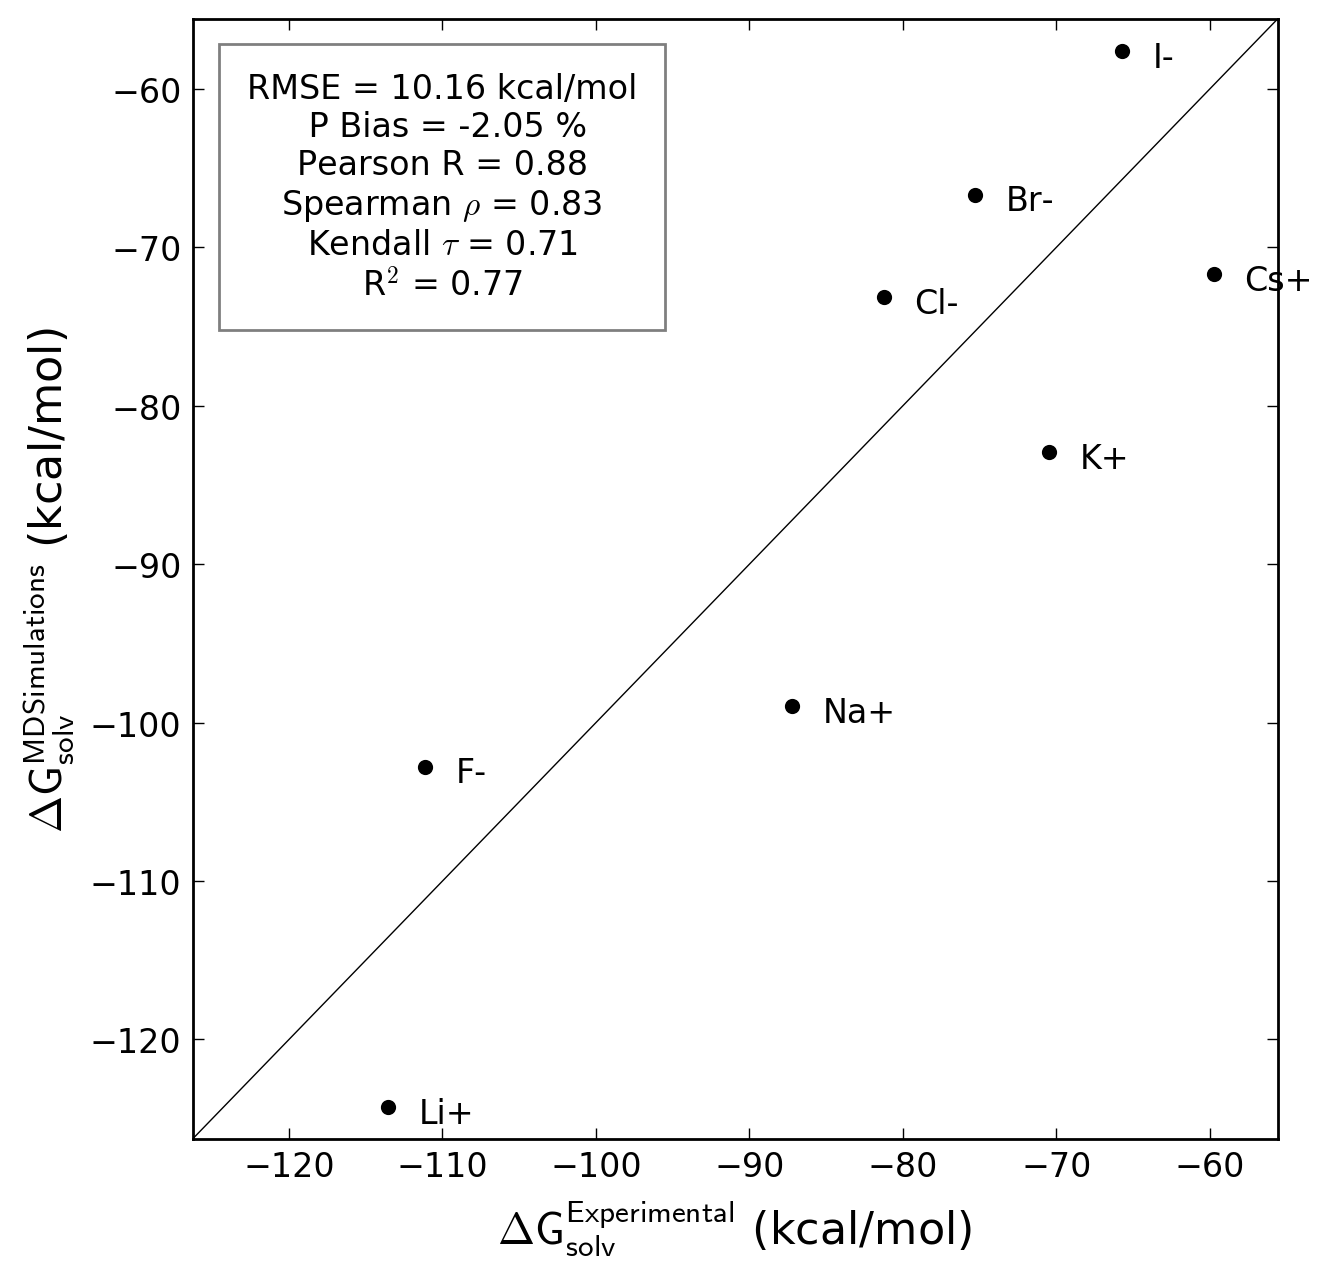
\includegraphics[width=\textwidth]{chapters/BDD/images/ions/MD_exp}}
          }
%       \caption{$\mathrm{m}_\mathrm{max}$=1}
%       \label{fig:distrib_error_PC_PCPlus:mmax1}
    \end{subfigure}
   \begin{subfigure}[b]{0.49\textwidth}
       \centering
       \resizebox{\linewidth}{!}{
         \fbox{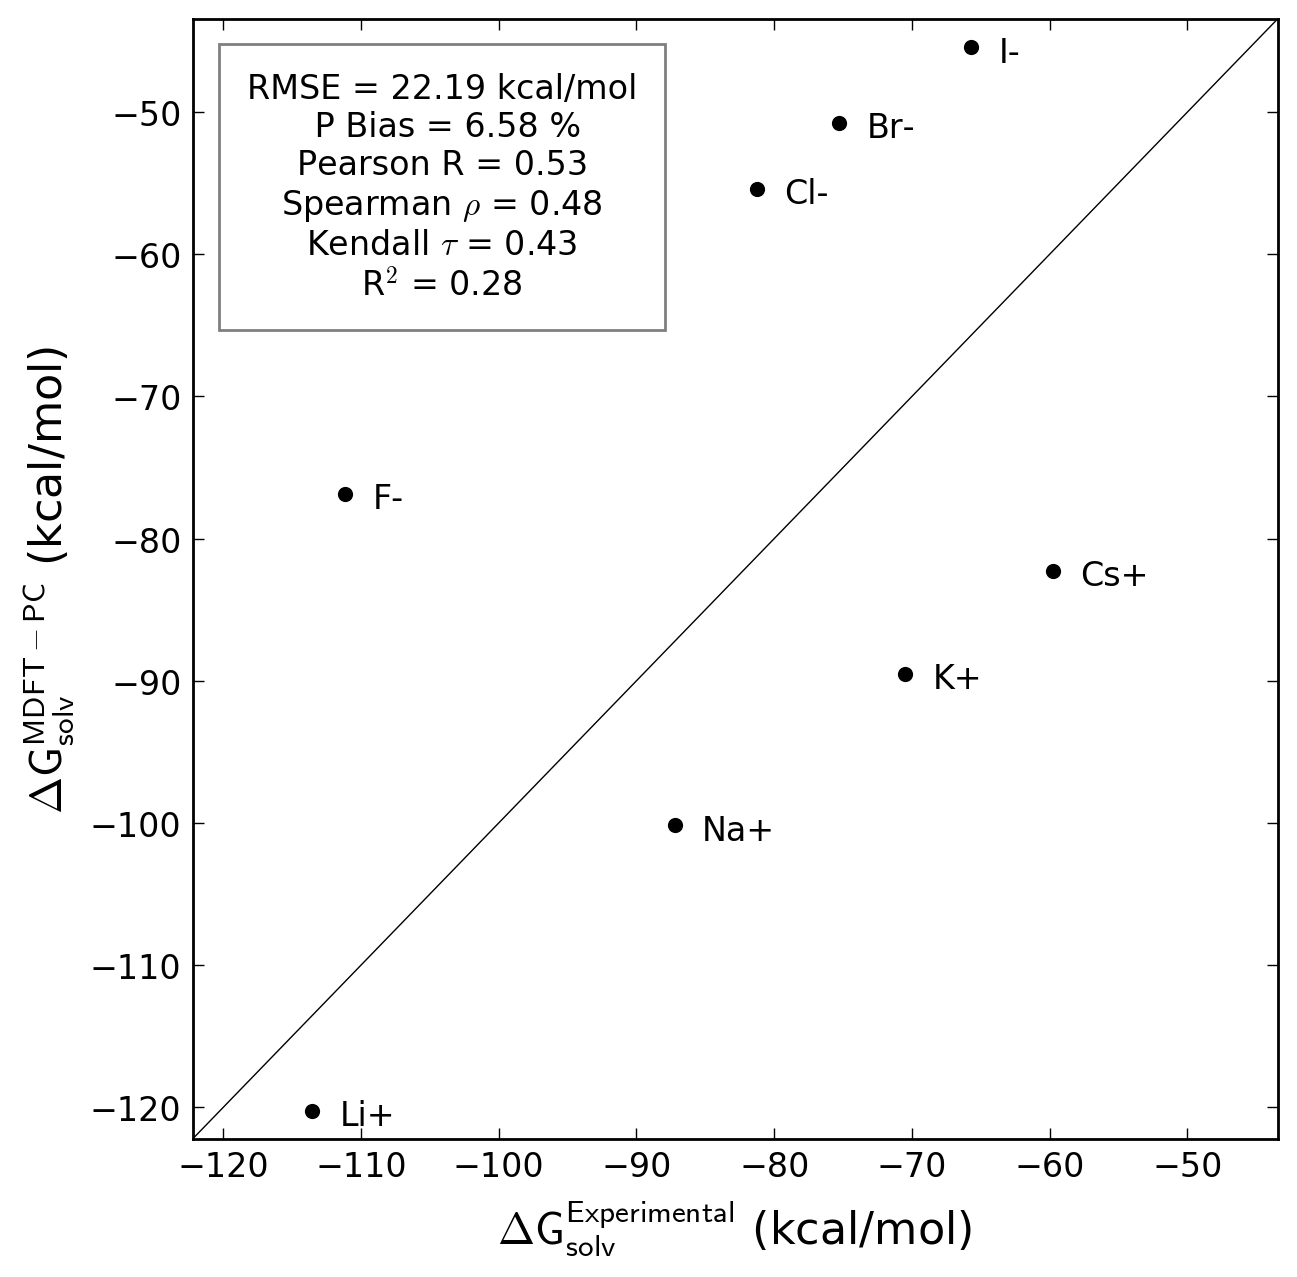
\includegraphics[width=\textwidth]{chapters/BDD/images/ions/PC_exp}}
         }
%       \caption{$\mathrm{m}_\mathrm{max}$=3}
%       \label{fig:distrib_error_PC_PCPlus:mmax3}
    \end{subfigure}
   \begin{subfigure}[b]{0.5\textwidth}
       \centering
       \resizebox{\linewidth}{!}{
         \fbox{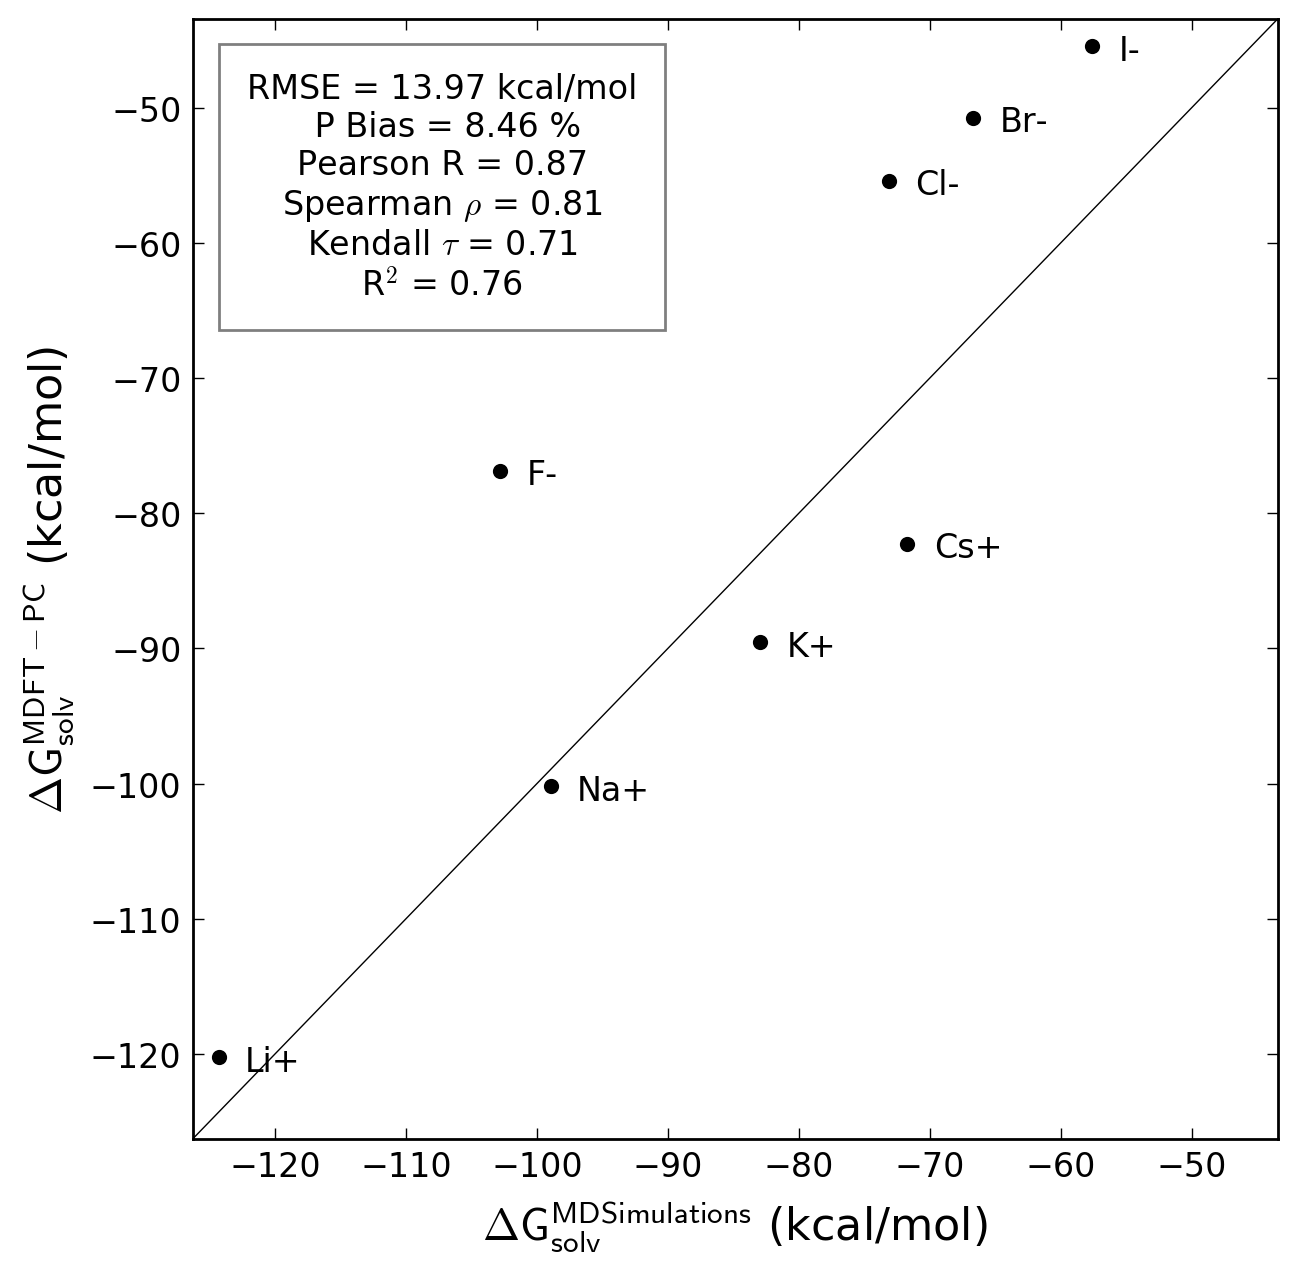
\includegraphics[width=\textwidth]{chapters/BDD/images/ions/MD_PC}}
         }
%       \caption{$\mathrm{m}_\mathrm{max}$=3}
%       \label{fig:distrib_error_PC_PCPlus:mmax3}
    \end{subfigure}
  \caption{Corrélation de l'énergie libre de solvatation calculée par MDFT, par dynamique moléculaire et expérimentales pour un ensemble de 4 anions et 4 cations.}
  \label{fig:correlation_ions}
\end{figure}




En ce qui concerne les cations, MDFT et la dynamique moléculaire sous-estiment de plusieurs kcal.mol$^{-1}$ leurs énergies libres de solvatation. Cependant, les résultats sont en accord pour les deux méthodes, ce qui laisse penser que le champs de force n'est pas adapté à ce type d'ions.

Au contraire, pour les anions, la valeur est sur-estimée de quelques kcal.mol$^{-1}$ seulement par la dynamique moléculaire et de quelques dizaines de kcal.mol$^{-1}$ par MDFT. La théorie de la MDFT n'est donc pas optimisée pour la solvatation d'ions négatifs. 

\boitesimple{
Cette étude nous à permis de détecter deux problèmes majeurs dans l'étude des ions. Dans les cas des composés chargés positivement, le champs de force ne semble pas adapté, alors que dans le cas des composés chargés négativement, la théorie MDFT est en cause. Ces résultats sont en accord avec ceux obtenus sur la base de données Freesolv. En effet, MDFT apparaissait le moins précis sur les composés comportant des hétéroatomes : les oxygènes et les azotes étant fortement chargés négativement.
}



\vspace{8\baselineskip}

\boitemagique{A retenir}{
Dans ce chapitre nous proposons un outil simple et efficace qui permet une analyse complète et reproductible de MDFT sur de larges chimiothèques. Nous avons dans un premier temps montré que la correction \textit{PC+}, plus adaptée au niveau actuel de la théorie, devait être abandonnée au profit de la correction \textit{PC}. Nous avons ensuite mis en avant certaines zones de l'espace chimique (charge partielles fortes, groupements hydrophobes) pour lequel MDFT manque encore de précision. Cette étude nous permet ainsi d'orienter les futurs développements théoriques de MDFT.
}


























